\documentclass[12pt]{report}
\usepackage[hidelinks]{hyperref}
\usepackage[english]{babel}
\usepackage[utf8x]{inputenc}
\usepackage{apacite}
\usepackage[a4paper,width=155mm,top=25mm,bottom=25mm]{geometry}
\usepackage{epigraph}
%\usepackage{setspace}
%\doublespacing
\usepackage{graphicx}
%\graphicspath{ {graphics/} }
\usepackage{caption}
\usepackage{subcaption}
\usepackage{wrapfig}

\setlength{\epigraphwidth}{.6\textwidth}
\setlength{\epigraphrule}{0pt}

\hypersetup{
    pdftitle			= {Thesis Draft},
    pdfauthor			= {Mustafa ilhan},
    pdfsubject			= {Trash, Art},
    pdfkeywords			= {mfa, thesis, trash, art},
    colorlinks			= false,
    pdfborder			= {0 0 0},
    pdfpagemode			= UseOutlines
}

% Quotation command
\providecommand{\quotes}[1]{``#1''}
\providecommand{\singlequotes}[1]{`#1'}

\begin{document}
\title{Thesis Draft}
\author{Mustafa İlhan}
\maketitle
\pagenumbering{roman}
\setcounter{secnumdepth}{3}
\setcounter{tocdepth}{3}
\tableofcontents
%\listoffigures
%\listoftables

%****************************************
% Title Ideas for Thesis 
% - Trash as an Artistic Medium.
% - Trash Notebooks: Trash in the Context of Art
% - Trash Notebooks: Exploring the potential of trash through art practice
%****************************************

%****************************************
% Abstract ideas
% You can add shortly definition of trash and discard. Any object can be art in 19th century.
% Structure of this thesis: written part of it and the project support each other.
%****************************************

\begin{abstract}
In this thesis (re-)usage of discarded materials in the process of art making and the artwork itself is explored (or researched). Why and how are they used by the artist? Are there any differences with the original items compared to discarded items? (In other words has using discarded materials or trash specific (or special) meaning and message?) This is a work to explore the re-usage of trash in artworks (place or the role in the art practice). (and also in which scope? medium, message, life practice\ldots) 

Actually (It is questioned that) working with trash dictates a life practice and, it is a convergence of behavioral patterns (attitudes toward to trash) and art making. The process effects how one's lives and lifestyle. (But what type of interaction between life and art making process?) (This claim is the main driving force of my artwork which is part of a thesis.) The purpose do not build a thing that is produced from discarded material to watch it from a distance. The important thing is to interact with it. Because it is already discarded (disgusting, abject, unattractive etc.) and general behavior avoid from it, this work must change it. It must call the viewer to interact with it. (not only watch.)

% Olay sadece böyle çöpten bir şeyler yapıp insanların seyretmesi değil, mühim olan onunla iletişime, ilişkeye geçmek. Yani zaten uzak durulan bir şey, onlardan bir şey üretildiğinde izleyici gene uzağında duruyorsa ne anlamı kaldı ki? İnsanların bu işin aşamalarının bir parçası olmalılar.

With the help of art discarded things can be find a place in the society. (By the help of artistic approach things can be gain new values and meaning even if they are discarded and excluded from daily life (or society).) The relationship between value creation and artistic practice examined through the artworks that uses trash as medium.

From periods where manual labor and long struggle required in production process and materials are reused and transformed again and again, have reached to periods where production process speeds up and becomes more accessible. Consumption habits have changed radically and have created piles of trash that is not obvious how to reuse them. In this work the practice and process of reusing and transforming trash which is an alternative to today's existing production and consumption habits is investigated. Stages and expression of this practice is examined with my artwork in the context of art.

Do she/he want to take back (or revisit) the trash once thrown away? People do not want to think of what they throw away. Turning them to a things that worth to look again. How do artists reflect garbage and what are their tactics? What is the thing that add value to trash and what is the role of art in that?

With the help of art discarded things ---in the scope of thesis trash especially paper trash--- can be transformed beyond the other industrial (or technological) methods.

Using trash can not only understand in ecological perceptions, it also have powerful political claims. Or it should be examined in deeper levels beyond collage and assemblage, the medium itself has different meanings. 

Junk(or trash) can be seen as a resource that is fertile to new meanings, creations and aesthetics. Ignored and discarded nature of garbage when rethought becomes fertile resource. Trash as a resource (as a artistic material.)

\vfill\noindent\textbf{\textit{Keywords:}} trash(discarded objects), art, value creation, transformation.
\end{abstract}

%****************************************
% Sample abstract from a thesis:
% Bu çalışmada, ne kadar itici bir kavram olsa da, çöplük olgusunun çirkinlikten güzelliğe ulaşarak estetik bir haz uyandırması amaç edinilmiştir. Iticici gözüken bir konunun resim diliyle anlatımı ile tersine çekici ilginç bir sanat konusu olabileceğinin somutlaştırılması amaçlanmıştır. Sanatçı bir anlamda doğada yaşamda bulunan küçük ayrıntıları, sanatsal bir gözle yaklaşarak gösterebilendir. Resim için konu denince hep bildik tanıdık nesneler, belli bir düzenleme anlayışı (Natürmort) ya da idealize edilmiş konular, temalar akla gelir. Oysa önemsiz gibi gözüken itici karmaşık konular bile sanatsal kaygılarla ele ahnabilmelidir. Önemli olan, bu konalara estetik yaklaşım ve izlenen anlatım yol ve teknikleridir. Özgün baskı dallarından kazı resim (gravür) tekniğinin ele alınan konunun görselleştirilmesinde, anlatımında en uygun teknik olmasıdır. Çünkü her sanatçı kendi doğasına en uygun olan teknik ve malzemelerin olanaklarıyla kendini en rahat biçimde ifade etme olanağı bulur. Kendine özgü bir biçim ve anlatım diliyle dile getirmek gerçekleştirmek çabalan özgünlüğü yakalamak içindir. Bu çalışmada özgünlüğü yakalamak, çöplük olgusunun oluşturduğu dinamik yapı, objelerin biçimlerine bağlı kalmadan plastik dille görselleştirilmiştir. Seçilen teknik doğası gereği raslantısal tadlarada olanak vermektedir. Oluşturulan resimlerde durağan bir dengeden çok dinamik biçim ilişkilerine dayanan gerilimli bir etkinin yakalanması amaçlanmıştır.

\pagenumbering{arabic}
\chapter{Introduction}

%****************************************
% Structure of this chapter
% Section: explain the topic and its significance, raise curiosity, give same facts about it.
% Section: state the the purpose of this study, specify the focus of it.
% Section: overview of chapters and structure of thesis.
% Section: a note on terminology, clarification about the comprehensive terminology.

\epigraph{If I seem to be over-interested in junk, it is because I am, and I have a lot of it, too --- half a garage full of bits and broken pieces. I use these things for repairing other things\ldots But it can be seen that I do have a genuine and almost miserly interest in worthless objects. My excuse is that in this era of planned obsolescence, when a thing breaks I can usually find something in my collection to repair it --- a toilet, or a motor, or a lawn mower. But I guess the truth is that I simply like junk.}{\hfill---John Steinbeck, \textit{Travels with Charley, 1962}}

% Bence introductionda çöpün farklı şekillerde ele alınabileceğini bir şekilde göstermek gerekli. Burdaki genel geçer yaklaşımdan bahsetmek gerekli.

% Ele aldığımız çöp insanların çöpleri, günlük kullanımdaki çöpler. Çok da değerli olmayan yerine yenisi koyabileceğimiz çöpler. 

In this thesis work to understand the different aspects of trash is a key element. Because as scholars agreed on (ref required.) it is part of our life and daily practice and it is very common concepts from developed western societies to rural areas, from disaster areas to \ldots(something beautiful here). Sometimes it is accepted as a problem (waste crises, ecological problems.) that is need to carefully and seriously managed. On the other hand it is accepted as a source of diversity. (To establish a solid understanding for trash, it is important to see its dilemmas (it is really a dilemma?)). Therefore we should ask these questions: What is trash? How does it became trash? Is it a end product or a source material? How much is it valuable? How much is it dangerous?

Western societies from periods where manual labor and long struggle required in production process and materials are reused and transformed again and again, have reached to periods where production process speeds up and becomes more accessible. Consumption habits have changed radically and have created piles of trash that is not obvious how to reuse them. In this work the practice and process of reusing and transforming trash which is an alternative to today's existing production and consumption habits is investigated. Stages and expression of this practice is examined with my artwork in the context of art.

In previous ages (pre industrial ages? which age?) objects and resources are used again and again. Production of objects are hard and laborious. \comment{Böyle çok fazla kullanılan nesneye örnek bulsak ne kadar güzel olur. Mendillere bunlara örnek olabilir. Aslında tam benim konumla ilgili çünkü tek kullanımlık. Hijyen kavramıyla ilgili giderek artan da bir ilgi necesiyle tek kullanımlık peçeteler gittikçe önem kazanıyor.} \todo{Susan Strasser}

% Trash is everywhere and, produced every time
Modern (developed) societies are continuously generating trash and, pile them on landfills. It's a common object category that all people share its possession (It is experienced by everybody.). During daily activities trash is generated and people get rid of them by throwing away. (Various objects become trash after their primary functions daily. Who defined the primary function? Primary function is the only function. People cares the package of the objects that they buy. They buy the coffee not the cup of it. After coffee finished the life of cup also finishes. There is a lifetime defined (or forecast) by the producer of objects. However it is not bound to the producer, also consumer play an important role. There are different choices. Throw it away. Keep it. Give it. Mostly wining choice is throwing away and by the result of it mountains of garbage are increasing.) The vast amount of industrial discarded items spread through the landfills to oceans. They are the result of highly complex industrial production methods. They are not easily disposable items. They live in the nature thousands of years. They are durable(in terms of resistant to natural affects) products. Most of them packages that are used to carry or protect other materials. After real material used these packages became valueless (or useless). (types of trash can be mentioned here, but currently in the artwork I'm using paper packages, therefore, it is more important.) How manage the all this increasing trash that damaging nature?  This is the common approach to trash and the main problem. (actually the sustainability problem.) It is not the only problem, It can be thought that it is a losing the ability to transform new things, alternative behaviors etc. (Instead of creating new opportunities or alternatives, it is a consuming all them and producing huge pile of trash.) (reference Zizek idealization of nature, to love nature is to love trash. Live with trash. Do not see it as trash actually. Then the question is how to love trash? how to live with trash? can living with our trash enrich (our perceptions, abilities)? how not to see them as trash and useless? Can it be possible with art?)

% FROM Trash as Treasure, BY WILLIAM L. FASH AND E. WYLLYS ANDREWS, ReVista
% TODO PRAP. REF.
\todo{Facts about trash} \paraphrase{Waste pickers are an important part of the story in Latin America, as more is being thrown away than ever. The World Bank estimates that the amount of solid waste generated in cities is growing faster than the rate of urbanization. The higher the income level and the rate of urbanization, the greater the amount of solid waste produced. OECD countries produce almost half of the world’s waste. Africa and South Asia produce the least waste. High-income countries have the highest collection rates and are most likely to dispose of waste to landfills or incinerators. Low-income countries have the lowest collection rates and are most likely to dispose of their waste in open dumps. However, low-income countries also have the largest numbers of informal waste pickers who collect, sort, and reclaim recyclables---thus reducing costs to the city and to the environment.}

% From Beautiful Trash Art and Transformation BY PAOLA IBARRA, ReVista
% TODO PRAP. REF.
\paraphrase{We relate to garbage daily. We use it, produce it and dispose of it. Endlessly. The most obsessive of us get rid of it as fast as we can. The hoarder likes to salvage a few things for later use---the plastic and glass containers, the cardboard boxes. We know that capitalism’s escalating cycles of production, consumption and obsolescence keep worsening an already problematic relationship between humankind, waste and nature (not to mention social and economic relations). Despite a relatively increased awareness about consumption and its consequences, the pace at which we also acquire and dispose of material objects is exploding. Particularly in the connection between garbage and the arts, I am interested in two questions. First, the issue of recycling as a general practice in the arts; and secondly, in the whole issue of representation---that is, representation of waste as subject, and representation (of waste or others subjects) through waste as material.}

% Konunun dikkat çekici ilginç kısımları. Interesting points of the topic. Facts about the trash. Changes through the time.
% Konu hakkındaki temel bilgiler.
% Konunun ele alınan kısmı.

% Çöp ve dönüşümden bahsetmek gerekli. Çöp nedir? Dönüşüm nedir? Çöpün bir dönüşümü var mıdır? Var ise bu nasıl bir şeydir? 
% Introduce as an discussion. Trash is valueless? really? is it just a sculpture? Tons of different approaches to the trash. 
People tend to think that trash is values because it is trashed no longer needed or not wanted anymore. However is it really values? What does make it valueless? They do not think what happens after they throw it away. It exits from your life but not the world. What happens when you throw away a It is stacked from another place. Value of objects are not static. Trash is not static also It has a long journey. A project conducted by MIT researches journey of trash by placing trackers onto the trash. The results are surprising. Trashes spread away across the country and this journey takes month. \todo{give exact reference} We know that it is not limited with the border of America because it is the one of the countries export their garbage to the other countries --- fourth world countries\todo{footnote what are these countries?}. In other worlds Americans trash is not only their trash. As commodities spread to the every corner of the world, trash also. What happens when it is traveled to the other countries, how they approaches these items. \comment{They find new uses and meanings on them.} \todo{consider Papua genen people}

% Cycle of trash
Trash moves, objects moves from place to place. From homes to garbage trucks. From streets to land fills. From garbage baskets to sculptures. [REF. MIT Garbage project] Lots of different people touches to trash. With the trash what moves?

Even if people pay little attention, everybody do not. An artist takes photos of his every trash, like people take photos of their faces. He focuses on the thing that paid little attention, that is trash. At the end he exhibits all the photos by covering all the walls of room. It can seen as record of his activities, record of commodities. Most of them we are not aware of them. Draw the attention of is being thrown away and everytime and everywhere. They are too much and can only fit covering all the walls. \todo{artist}

% Bu trash in every sıralamasını neden yapıyorum? Genel bir çerçeve çizmekten çok aslında evrensel bir konu olduğuna değinmiş oluyorum. Peki bu çok açık bir şey mi? Yani aslında çok da açık olmayan bilgilerek vererek yaparsam olmayabilir. Evrensel olmasının benim için ne önemi var. Yaşamımızın bir parçası demek. Tamam da buna karşı bir şey mi var. Ben göremiyorum açıkcası. Herkes bunu biliyor. Farkında mıyız. Ama farkında olmak istemediğimiz bir şey ki sürekli kendimizden uzaklaştırıyoruz. O zaman bu gerçekleri aslında ne kadar biliyoruz. Ama bunları bilmek böyle davranmamız gerektiği anlamına mı gelmektedir? Aslında yabancı olmadığımız ama uzak durduğumuz bir konu. Belki de sırf bu yüzden kaçırdığımız bir sürü şey olabilir.

Trash is global, and shared concept for all societies throughout the ages. 
\textbf{Trash in every age.} In other words it is part of human activity of every historic age. It exists early ages of human to now. Trash is part of the early days of human production / or activity. Firstly the word garbage is actually used for the parts of animal that cannot be consumed by the human. Legs, bones etc. [TODO etymology reference, see appendix] Archaeologist find things from people throw away. 
\textbf{Trash in every society.} Some of them called as trash the others don't. Somehow all actions of people generate trash. It is common. 
% TODO look introduction of revista, there is a related reference above it.
\textbf{Trash is everywhere.}

% ARTWORK
% Sad chair http://www.keaggy.com/chairs/sad/12/. Photos of lonely chairs that are no longer wanted. Artist captures the continuous 

Why people are interested in rubbish. Some of the artist also interested in others trash. \comment{O çöplerde ne bulmayı umuyorlar ki? Aslında çöp bizim davranışlarımız, yaşayız tarzımız hakkında bize yön veriyor. ve bu her zaman fiziksel dönüştürme ile değil de aynı zamanda anlamsal ve mekansal değiştirme sorulamalarla mümkün oluyor. Bazen de olduğu gibi kullanıyorlar. bu açıdan önemli. Çöpü çöp şekliden sunan sanatçılar. Ama bu nasıl mümkün ki? fotoğrafını çekenler aslında gerçekten ona müdahele etmemiş mi oluyorlar. Bence değil? bir şekilde müdahele var gene orada. o fotoğraflarda artık dikkatin objesi haline geliyor. çöpün dönüşmesi aslında bir diğer yandan çöpe bakışın değişmesi olarak görülebilir.

% Amelie olabilir. Orada fotoğraf toplayan çocuk olabilir. Onları itinayla toplayan bir adam. Tren garındaki fotoğraf kulubesi. Belki de dünyanın dört bir yanından gelen insanlar, bir kesişim noktası. Bir birinden farklı bir sürü insan. Filmde neden böyle bir eyleme yer veriliyor? Film fotoğraflar üzerinden defter üzerinden ilerliyor. Onun çevresinden bir hikaye kurgulanıyor. İnsanların artıklarını topluyor. Onların değer vermedikleri şeyleri topluyor. Bunlar baya baya aslında o insanlar. Bazı fotoğraflar çok fazla küçük parçalara ayrılıyor. Çok iyi bir örnek mi bilmiyorum. Burada niyet nedir ki? Ben buna şöyle bir okuma getireceğim diyebilirim. Amelie mesela küçük ayrıntılara dikkat eden bir insan, bu fotoğraf taplama işi de aynı şekilde. Bu arada bu fotoğraf toplama işi ilk değil. Found photos diye başka bir paper var ve orada aslında bu işin ilk uygulaması gösterilmekte. Ama benim işime yarayan kısmı ne? Neden o fotoğrafları ya da bunun filmini yapıyor. Aslında puzzlelar üretiyor. Belirli tekrar olacaktır. insanların kapalı bir ortamda nasıl pozlar verdiklerini sonrasında ise onları attıkları şeylerden görülebilir. Tekrar bir kitap haline geliyor. Tanınmayan insanların fotoğrafları. Nerde oldukları, neden ve nasıl çekildikleri belli olmayan bu yüzden aslında ilişkilerin insanlara bırakıldığı bir koleksiyon. Aslında tam da amelie bunu yapmıyor mu? Hikayeler üretiyor bu fotoğraflardan. Yeni karşılaşmalar üretmesi. Her ne kadar sıradan portre fotoğraflar olsa da birbirlerinden oldukça farklılardır. Bin bir türlü şey vardır aralarında. Nereye yerleşmeli. Başkasının çöpünü toplama. O dönemin o eşyasını arşivini tutma. ve herkes sunuluyor sonrasında bu.

% Wall-E belki olabilir. Dünyanın aslında bir çöp yığını haline gelmesini gösteriyor olabilir. Çöp dağları, çöp denizleri. Atılmış binbir türlü nesne. ve wall-e ise bunları ne yapıyor sadece pressleyip bir kenera bırakıyor. Bundan basetmişken aslında pressleme işi yapan şu cesar. Bu şekilde olmak zorunda mı? Bunun alternatifi yok mu? Aslında bu tezde bunlara cevap bulunabilir. Çöpe olan bir sürü yaklaşıma ek olarak bir de bunlar var. Ya da başka neler var? Bunları araştıran inceleyen bir yazı. Wall-E'nin çizdiği portreyi tekrar ele alırsak ne görürürüz. İnsanlık buna mı dönüşücek? Başka bir ihtimal yok mu? Gerçekten de dünyayı bekleyen şey bu mu? Bir çöp yığını olması mı? Bu bir abartı mı yoksa gerçeklik payı yadsınacak cinsten mi?

WALL-E is a 2008 American computer-animated science fiction comedy film produced by Pixar Animation Studios. A robot named WALL-E, who is designed to clean up an abandoned, waste-covered Earth far in the future. WALL-E resembles giant dozers that moves and piles trash in the landfills. This robot creates squeezed trash blocks that have no meaning and interpretation. All different objects in terms of their physical and social properties turned to same squeezed garbage blocks. There are mountains of trash and place is very limited. By squeezing them, WALL-E saves space. \todo{What is the context of it? Which part is related with my topic?} What are we going to do with all these mountains of trash? \todo{Can it be placed under zizek part?} WALL-E represents a possible future condition of Earth.

% TODO Life time of objects.
% Nesnelerin yaşam süreleri, Bu yaşam sürelerinin ne kadar olduğu. Burada ilginç bilgiler olabilir. Aslında ne kadar çok üretip ne kadar kısa sürede tükettiğimi görüyoruz. Ama eskiden ürünler daha uzun sürelerde kullanılıyordı. Sonrasında ise bu kısa sürede tüketilen ürünlerden nasıl dağlar oluşuyor. Çöpçü kaç günde bir ziyaret ediyor. Çöp kutuları ne kadar sürede bir doluyor. Çöp kovalarının içlerinde neler var.

\todo{Background information about the thesis. Inspirational points. The fact of trash.}

% Şöyle bir şey var, sanata non-art objelerin girmesinden bahsediyoruz ama artık orda o seviyede değiliz. O zamandan bu zamana çok şey değişti. 
\comment{In the beginning of the 20th century non-art objects enter the scope of art making. This is a revolutionary change in the making of art. Production of art and the approach to the art changed dramatically. This changes actually started at the end of the 19th century with impressionist. (But not related with non-art objects.) Picasso is the first artist that used non-art object in his works. Later many of them followed him. First works are collage which gluing different papers together. Yes using non art objects in the art is introduced and opened new dimensions for the language of art. But some of them treated as sculptures from trash. Reflects our world. But it is not limited with this. Some of the works are provokes the consumption habits of society and offers an alternative perception.}

% Aga çöpe farklı yaklaşımlar var. O yüzden background information olarak burada verilebilir ve scope belirlenebilir. Tam da bu noktada ise purpose kısmına geçilebilir. Çöpe nasıl yaklaşıyorlar falan filan. İşte ben tam da bu noktada sanatta nasıl yaklaşılmıştır dicem. Hatta basitçe sanatta bu tür işlere 

\comment{Trash draws attention different peoples and disciplines. In other words there are different studies related with trash. Different approaches to the trash and son on. However in this thesis study trash }

There are many works from trash around the world. Build up trash. Collected from graveyards, landfills, unused materials etc. 

% Aslında sadece bir heykel işi olan şeylerden bahsedebilirim, ya da aslında belki de içine girip dokunabildiğin bir şey olabilir. 

% Savunma.
% Yani aslında bu chapterdaki fikirler vs.'ler birer supportive yaklaşımlar. neler yapılmış onları listesi. literatür taraması. ama tabi benim işime yarayanlar. 

This trash pheomanan catches the attention of artist. It is very human activity. In this context which trash? What type of discard. Many type of it?

% Idea of everthing can be trash. Act of trashing. not act of transforming. Trash is like kara delik gibi ışığın odan kaçamaması gibi hiç bir şeyin ondan kaçılmayacağını hissediyor aslında. 
% Michael Landy's Art Bin uses a art gallery to create his dust bin. Describing the work, simply called Art Bin, as 'about failure', Landy is inviting members of the public to bring their own artistic failures along to the gallery from 29 January, where their worthlessness will be assessed. Damien Hirst, Gillian Wearing, Tracey Emin and Mark Titchner have already contributed, offering sculptures, paintings and prints. "There's no hierarchy once they are in the bin" All of them are accepted as same. Ultimate equality. Tosing them to the dust bin makes them rubbish even if they are combined from failed attempts. Nothing's too good for the art bin. Everything can fit into the art bin. Michael Landy transforms the SLG into Art Bin, a container for the disposal of works of art. As people discard their art works the enormous 600m³ bin becomes, in Michael Landy’s words, “a monument to creative failure”. It is a very big glass bin and isolates people. There is a provocative approach to the art and art objects by saying that "Nothing's too good for the art bin". There is no limitation of throwing away even if art. 

%%%
%%%
%%%
\section{Purpose of the Study}

%****************************************
% It is a justification of the work. 
% What is trash? Who does call it trash? 
% Is it possible to transform it? How? Which methods?
%........................................

\todo{what do you mean when saying ``transforming trash"? Needs to be opened. I claimed that such a thing exist? when it is exist? by physically or conceptually? actually both of them exist.}

% Bu söylemeden önce insana böyle bir şeyin mümkün olduğunu anlatmak gerekli. Yani aslında transformation of trash diye bir şey var aga demeli. Kimler bunu nasıl yapmış. Neler var ortalıkta bunlara bakmak gerekli. Pres makineleri falan. Ama bunu aynı zamanda sanatsal açıdan inceleyenler, sanatsal amaçlarla yapanlar bulunmakta demek gerekli.
The aim of this study is to explore the theories and methods in transformation of trash in the context of art and artistic act.

In this thesis (re-)usage of discarded materials in the process of art making and the artwork itself is explored. Why and how are they used by the artist? Are there any differences with the original items compared to discarded items? Has using discarded material or trash specific (or special) meaning and message? This is a work to explore the re-usage of trash in artworks (place or the role in the art practice). (and also in which scope? medium, message, life practice\ldots) 

% Çöpün sanat işlerinde kullanılmasının önemi ne? Bunun karşısındaki şey nedir? Diğer alanlardaki yaklaşımlar bir şey üretemiyor mu? Bu tezin önemi ne? Birilerinin bıraktığı boşluğu doldurmak mı? Ya da benim yaptığım işin önemi ne? 

% Önceki işlere değinmek gerekli. Bu alanla ilgili yapılmış. Mesela ne var. İki tane tez buldum aslında tam da bu konuyla ilgili. Önceki işler olacak, yetersiz eksik yanları olacak ve ben onlara belli başlı eklemeler yapacağım.

As many people are inside the business of transforming trash through craft and so on. People on the streets looking for aliminu cans, glass bottles, plastic. They collect and sell them to survive. There are companies that are collect waste materials to regain them again the industry. In thesis they are not in the scope. People that give attention to the trash and behave artistic act is in the scope of this thesis.

% How does it become trash?
Here the purpose is to understand the dynamics that turn objects to trash. By understanding them is provide a roadmap (or ideas) how to turn trash to something valuable? (The purpose of this thesis is to find (or explore) a way(methodology, approach) to add value to object using artistic methods? Therefore first question is why they are less-valued, and ignored. How to make them valuable? How to make them part of our life again?)

%%%
%%%
%%% 
\section{Overview of Chapters}
This study is structured many examples of artworks in different part of the thesis. As the related topic or argument is presented example artwork is given at this moment. Immediately how artist replies this issue is illustrated. Thereby artworks are examined in the theoretical and cultural context. Art works are used as a supportive elements for the stated arguments. \comment{yeri geldikçe de gene bu işlere ele alınmış farklı açılardan incelenmiştir.}

Following chapter ---Trash in Culture and Theory--- explores the place of trash in the cultural life and theoretical approaches on trash. The aim is (better) to understand the trash in cultural and theoretical aspects. (to better realization the notion of trash.) It is explored the trash is being worked is whose trash. Or what type of society genarete this trash. Also in the project I collect the paper trash. What type of approach generate it and what are the dynamics of it? What type of trash we are talking about? It is understood through the patters of consumption patterns. And to reflect this cultural phenomena what phylosphers and scholars say. Artist how they are reflected this notion.and also looked how scholars are conceptualized trash and its movement on the different values system. How explained the transient nature of trash?

\comment{First chapter will be about the conceptual framework that I have been working through
which includes historical and theoretical background.}

Third chapter seeks the root of using trash in the artworks and looks through the sample artworks. As already artworks are mentioned in the different part of the thesis, in this chapter focused on art (historical )

Fourth chapter explains the project that supports this thesis. Its stages and approaches to the topic mentioned here.

\comment{The second chapter will consist of the overview of my work. I will start with the development process of the work. I believe that the way an artist works and the obstacles that she encounters have a huge impact on how the final work is embodied. Development process of my work shaped the way I think on the subject of my thesis. Therefore, I will explain my process as detailed as possible. Then, I will continue with different aspects of my work; formal decisions and usage of light that I believe carry my work to another level. At the end of this chapter, we will see how my work functions and what it proposes on the image and word relationship.}

Finally last chapter offers an overall conclusion of this thesis and project. 

%****************************************
% About the thesis statement and focus:
% Is it too broad?
% Is it debatable? Is is fact? (Trash is not a end point of objects, there is a life waiting for them?)
% What is my side? throwing away is required for society to go further? or omitting the tons of possibilities... 
% Supporting claims?
% What is my thesis statement? Again same topic... It needs to be solved...
%........................................


%****************************************
% Sample phrases:
% The discussions (mentioned discussion are also formed the thesis project entitled ... )
% Aim of this thesis is ...
% There has been a recent spate of artistic work focusing on (over-)consumption using the lens of disposal and discard.
% as a reaction to the consumerist society.
%........................................


%****************************************
% Some comments
% Burada önemli olan şey soru veya sorgulanan şey. Bu soru projeye yön verecek. Yazılı tez ise bunun doğrulamasını, üretilen işin kavramsal ve kuramsal çerçevesini belirleyecek. Tartışmalar ne üzerine olmalı bu durumda? 
% The project aims to what? and what needs to justify what it questions? 
% At this point, the question of what will be in the future of photography has to be asked. Bu çok önemli, bir şeyler hazırlayıp neyin sorgulanması gerektiğini sormak gerekli.

% Tipografi ve ideoloji arasında bir ilişki vardır. Fotoğrafın geleceği? Kelime ve imaj arasındaki ilişki, beden ve algı üzerinden incelenebilir? kelime ve imaj arasında bir problem olduğundan bahsediyor. Sanat işlerinde çöp kullanmak toplum tarafından atılan şeyi tekrar kullanılabileceğini gösterebilir. Toplum ve çöp nispeten bir problemli bir durum. Burada bir dert var. Atılan tüketilen manalar var. Sanat bunları provoke mi ediyor. Peki ya ben ne öneriyorum, yani aslında bir şey önermem mi gerekiyor? Sanat ve çöp arasında nasıl bir ilişki vardır? Çöp ile diğer nesneler arasında nasıl bir ilişki vardır? 

% Zaten hali hazırda sanatçılar bunu yapıyorlar, tez aslında bunları inceliyor olabilir ama tez aslında benim işimi inceliyor. İş neyi soruyor ise aslında tez de onu soruyor. Yapılan işlerle sorulan sorular arasında bir bağlantı var. Bu noktada aslında benim işin neyi sorguladığını bulmam gerekli. Çöp dönüştürülebilir, sanatsal bağlamda. (Çok geniş değil mi abi sanatsal bağlamda demek? Çöp de çok geniş bir konu.) Konuyu bir şeklide daraltmak gerekli. Çöp sanat işlerine girmiştir. Çöp dönüştürmek aslında bir artistic acte dönüşüyor. Tezde bunu anlatıyor. Aga bu artisctic act dediğin şey de ne oluyor. Çöp dönüştürmek ne oluyor?

% Çöpe yeni bir alternatif yaşam üretmek gerekli! Neden böyle düşünüyorsun? Çünkü sürekli çöp üretiyorsun ama bir yandan da bundan dert yanıyorsun. Zizek işte bu konuya el basıyor. 

% Aslında hepimiz bir şeyleri dönüştürüyoruz! Neden böyle düşüyorsun? Örnekleri nelerdir? Bricologe bu iddayı destekler mi? Nesnleri üretim amaçlarından farklı amaçlar için kullanmak yeni bir şey değil. (Ama zaten ben sanat amacıyla kullanılmasından bahsedeceğim.) Belki bunu belirtmek için mantıklı olabilir. Ama burada bir farklılık var olamalı. Diğerinden ayıran diyeceğim ama öyle bir fark aramamak gerekli bence. Sanat o farkı yıkmak için uğraşıp duruyor. Belki de bu uğraşa katkısı bu olabilir bu işin. Bir şeyleri dönüştürme potansiyellerimiz olduğunu düşünebiliriz. Dönüştürme dediğimiz şey aslında hangi noktada açığa çıkıyor. Bir ihtiyaç anında, kaçış anında, ya da yeni alternatifler ararken mi?

% Çöpün dönüştürülmesi ne olaki? Buna bir şekilde girişte yer vermek gerekli. Çöpün market içindeki hareketi mi? Ya da aslında çöpün yaşamı. Belki de bu olabilir. Çöpün nasıl oluştuğu vs. Fabrikada üretilmesi. İnsanlara dağıtılması. Ve sonra çöp olması. Çöp dağları oluşması. Çöp kutusunda yer alması. Neler yok ki çöp kutusunda. Bir sanatçı çöp kovasına attığı sanat işleri. Sanat işleri çöplükleri vs. Çöp kavramı aslında o kadar çok şey için geçerli ki? İşte bu çok çeşitli çöp kavramını ele almak gerekli. Yani objeler bir şekilde farklı konumlarda mekanlarda yer değiştiriyorlar. Bazen çöp oluyorlar bazen değerli vs.

% Bir bir çeşit çöp var. Bunlar binbir çeşit davranış sonucunda oluşuyorlar. Bir işlemin sonunda ortaya çıkan son ürün. Çöp konumuna gelmesi vs. Kime göre çöp neye göre çöp. Ama işte ortada bir konsensus yok. Başkaları da farklı şekilde görüyor. Birine göre çöp diğerine göre ise bir hazine.

% Dönüşmek ne oluyor peki bu durumda. Bir durumdan başka bir duruma geçmesi. Farklı bir anlam, amaç kazanması olabilir mi? Mesela pisuvar dönüşmüş müydü? Gazeteyi kolajda kullandığım zaman gazeteyi dönüştürmüş mü oluyorum? Hangisi dönüştü? Zaten buradaki açık bir şekilde açığa çıkıyor aslında. Her ikisi de dönüşmüş oluyor. Farklı bir kullanım alanı bulmak. Farklı niyetlerle kullanmak olabilir belki de. Bir şeyin ne zaman dönüştüğünü iddia edebilirsin.

% Agnes varda neyi anlatıyor: Toplayıcılık hala devam ediyor, bu toplayıcılar arasında sanatçıları da geziyor, çünkü onlar da topluyorlar. Onlar da o çöplerde farklı şeyler görüyorlar. Kendi de mesela çöpe atılmış bir şeye anlam yüklüyor. Kendisininde aslında bir toplayıcı olduğunun farkına varıyor.


%****************************************
% JUSTIFICATION (Gerekçesi)
% Eğer bir şeyin justificationından bahsediyorsak ben neleri iddia ediyorum:
% - Çöpü dönüştürdüğümü. Öncelikli olarak o gerçekten çöp mü? Sonrasında ise gerçekten dönüştü mü? (throw away culture çöpü anlatsa. rubbish theoryde dönüşümü anlatsa)
% - Peki neden bu işi yapıyorsun. Alternatifi aramak. Değer bulmak, değer bulunabilceğine inanmam aslında. Belki de değer üretmek için o değerleri yıkmak gerekli. Çöpe atıldığında bu yüzden bazı değerler yıkılıyordur. Artık yeni değerler vermek için gerekli yapı oluşuyordur o zaman. O yüzden çöpe atılması önemli. Bir yerin sonuna gelmiş olması aslında belki de yeni bir başlangıç olması için önemli olabilir. Çöplüğün bir başlangıç olması. Batırdığımız bitridiğimiz yerden yeni bir başlangıç. Çöpü üreten üretilmiş şeyleri bitiren zihniyetle tekar düşünmek. Aslında çöpe baktığında üretilen şeyin ne olduğunu tekrar sorguluyor olabilirsin. 
% - Çöp sanat işlerinde kullanılabilir. Bunlarla ilgili örnekler var.
% - Çöp bu sanat işlerinde dönüşmüştür. 
% - Elimdeki literatürden belli başlı argümanlar çıkarmalı, bu argümanlar benim yaptığım işi destekliyor demeli:
%........................................


%****************************************
% SANATTAKİ KÖKLERİ ÜZERİNE:
% picasso falan gibi adamların derdi sanata farklı objeleri sokarken ki amaçları ya da değerlendirildikleri nokta farklı bir şeyler yapmaları. O dönemki anlayışı yıkmaları. Onun yerine daha geniş bir alan imkanı sunmaları. Biz şu anda onların açtıkları alandan top koşturuyoruz bir nebze. Onların buna yaklaşımları ile bizimkiler arasındaki bazı farklılıklar olacak. En azından biz onların yıkları şeyi yıktığımız iddia edemeyiz. Çünkü o kalıplar, yaklaşımlar açıldı ve yeni bir üretim alanı insanlara sunulmuş oldu. Sorulacak yeni sorular, yapılacak yeni tartışmalar vardı. 
% Yani farklı dönemlerde farklı amaçlarla kullanılmıştır. Farklı şekillerde okumak mümkündür. Ama benim işime yarayanları seçmek gerekli bunları. Bir kısmı için bu sanatın diline yeni bir şey sokması, sanatın alanını genişletmesi, yeni tartışma alanları açması şekilde işime yarayacak. Diğerleri ise çöpe ele almaları 
% Ben picassonun sahip olduğu kaygılarla sanat yapmıyorum. Yani ondan bahsetmek ya da sanatın bu işlerdeki köklerinden konuşmak benim için yeterli değil. DAha da fazlasına ihtiyacım var. 
% Benim kaygılarım ne peki? Ben kime hitap ediyorum, bence burada bir ayrım söz konusu.
%........................................


%%%
%%%
%%%
\section{A Note on Terminology}
(Garbage, trash, rubbish, debris, detritus, waste, scrap, junk, refuse, discard, disposal, litter: during my research scholars and authors have different names for the stuff.) I realized that many scholars and resources have used different words (or terminology) to define trash. Although there are slight differences between these words, sometimes they are used to signify same concept (or used with same purposes). It is important to understand diverse vocabulary of this topic before dive into the theory. It is very important to choose right terminology, because ... and also make more clearer the borders of the work. There is no agreed (or specific) terminology. Some scholars uses junk art, others recycling art. Sometimes this make difficult to research on this topic. And also I must point out that this topic is not limited with the English language. The topic is broad and it is not limited with English literature and vocabulary (ref required). 

% FROM Rubbish! The Archaeology of Garbage, p.9
Several words for the things we throw away---"garbage", "trash", "refuse", "rubbish"--- are used synonymously in causal speech but in fact have different meanings. \textit{Trash} refers specifically to discards that are at least theoretically "dry"---newspapers, boxes, cans, and so on. \textit{Garbage} refers technically to wet discards--- food remains, yard waste, and offal. Refuse is an inclusive term for both the wet discards and the dry. Rubbish is even more inclusive: It refers to all refuse plus construction and demolition debris. The distinction between wet and dry garbage was important in the days when cities slopped garbage to pigs, and needed to have the wet material separated from the dry; it eventually became irrevelant, but may see a revival if the idea of composting food and yard waste catches on. We will frequently use "garbage" in this book to refer to the totality of human discards because it is the word used naturally in ordinary speech. The word is etymologically obscure, though it probably derives from Anglo-French, and its earliest associations have to do with working in the kitchen.

The origin of vocabulary of this topic reveals a whole side of human activity: our history revealed by what we have thrown away through the ages. What were people throwing out when these words were coined? 

%****************************************
% Reuse and Recycle
One of the most encountered words in this topic (transforming trash) is reuse and recycle. Both of them are used widely by scholars \todo{ref}

According to the dictionary, the word “reuse” means “to employ for some purpose” or “to put into service.” Reusing involves usage of the same product unchanged in form. If any item is used again and again over time, it is said to be reused. The main purpose of reusing is to lengthen the life of the item or material. Other examples are; buying some items and then selling them as used items, repairing some lawn equipment and reusing them, upgrading a computer, renting books, journals, periodicals, DVDs and others. The main purpose is to make the item last as long as it can. To reuse is to use something again instead of throwing it away or sending it off to a recycling company. Why throw something away when you can give it another life? Reusing is significant way to conserve and be earth-friendly because it keeps items out of landfills and reduces the greenhouse emissions caused by purchasing a new product. Using something multiple times -- like using a disposable container more than once -- is not the only way to reuse; you can also give old items a new purpose. For example, use an empty coffee can to store small craft supplies or an old loofah as a scouring sponge for cleaning sinks.

According to the dictionary, “recycle” means “to treat or process (used or waste materials) so as to make suitable for reuse.” In recycling an item, it is processed into a totally new product. It is an energy consuming process. For example, if we put some plastic bottles, paper, or aluminum items in a recycling bin, these materials may be recycled into a totally different thing as clothing items, fabric, or maybe a quilt. In this process, energy is required which depends upon the stages of transformation.

Recycling occurs when waste in an unchanged chemical form is used in the same process that created the original product. Examples are crushed glass containers (cullet) used to make new glass containers, and scrap metal used in foundries. 

Reusing is possible with re seeing (rethinking). Reusing is possible meet the needs of the human itself. Using creativity and personal approach can change objects functions. It is possible to use objects for different purposes. 

Recycling can be viewed as down-cycling. The object smashed to the small particles to be used later in the production of something else. Although reuse can be viewed as up-cycling that gives another (or more) value to the discarded products. Down-cycling does not generates new meanings it tries to convert the product to already known state to process. 

Recycling is very similar the rotting (decaying), reuse is something like dry tree branches used by birds for their nest. These are two agents of nature to regain their resources.

Many scholar used the word recycling when mentioning works use trash and the concept of it. However they are not mentioning the meaning that is decomposing things to the their particles. What they is actually is reusing and combining things, concepts, creating new mixtures.

%****************************************
% UPCYCLING TERİMİNİ KULLANANLAR.
% Burada da upcycling kullanıyor aslında. http://www.gwynethleech.com/cups/suspended
% Raw+Matrial=Art burda da upcycling deniliyor.
%........................................

\chapter{Trash in Culture and Theory}

% FROM Uncle Fernando’s Garbage Triptych, http://alphabet-city.org/issues/trash/articles/uncle-fernando-s-garbage-triptych, http://priscilauppal.ca/books/alphabet-city/
\epigraph{Anger is nothing compared to garbage:\\ Garbage eats anger for breakfast.\\ It eats all of us in the end.}{\hfill---Priscilla Uppal, \quotes{Uncle Fernando’s Garbage Triptych}}

In this chapter trash and the practice of transforming trash is examined in theoretical and conceptual aspect. Theoretical foundations of trash are discussed. Further benefited from historical and social aspect of trash. It is questioned that how do scholars conceptualized the trash, what do they say about it? 

Firstly we need to ask what is the source of trash. How is it generated? Secondly \ldots

%%%
%%%
%%%
\section{Throw away culture}
%%% Reference from Identity, mobility and the throwaway society
The term is actually a criticism of over consumption of short-live disposable objects.
\todo[inline]{We live in a throwaway society (Barr, 2004; Cooper, 2003, 2005; Cooper and Mayers, 2000; Strasser, 1999, cf. O’Brien, 1999; Hawkins and Muecke, 2003); (ref from another article)} whose behavioral pattern produce every time and everywhere. Even if conducted a qualitative research people are really do not throw away their things. \paraphrase{The research did not include the leftovers and detritus of food consumption packaging, bottles, and food waste, for example and neither was it concerned with another major category contributor to the volume of household waste, those `disposable' goods that are the primary means to maintaining bodily hygiene and cleanliness (Shove, 2003)}. They analyzed the things like television, furniture and toys like that.

\comment{Continuously consuming things and disposing of something. It is an important concept to understand why trash is trash? (or how it become trash?)}

(Our trash generating behavioral daily consumption patterns \ldots What are the results of them? Why are they throwing?) (There is a behavior that throws away and opposite of it there is a collecting behavior.)

\paraphrase{In this thesis the undeniable matter of waste, itself pressing, urgent and excessive, is used to infer the presence of a society defined by its generation; a society ceaselessly discarding and abandoning its surplus as excess, as part of an endless desire for the new. Morally corrupt and unequivocally environmentally damaging, the rhetoric of the throwaway society classifies discarding as intrinsically bad and commands us to assume control of our wasting, suggesting the adoption of heightened regulatory practices around disposal as the means to ensure that we clean-up our act. The thesis, however, lacks depth and provenance. It is, actually, glib. Indeed, to infer the presence of a throwaway society from contemporary levels of waste generation is problematic for at least four reasons.}

\comment{zaten zengin olanın atma lüksü var.}

\paraphrase{Life magazine fashionably heralded the advent of the "throwaway society" in 1955. 1971 daniel ingersoll reporting on his findings in the journal man in the notheast, "the industrial revolution ... was supplying the customer with hundreds of disposable containers and materials bt the end of the nineteenth century. the estimated 25.000 cubic yards of fill deposited in the upper portion of puddle dock show that the age of the throw away world began not in the twentieth century but during the nineteenth."} Therefore Industrial age played significant role (engine of the mountains of rubbish.)

% Resource is here: mmmacleo2005.pdf (throw away culture ile ilgili.) (Çünkü ben bunun ürününü kullanıyorum.)

\comment{All around of us filled with the things that are disposable. They are part of our daily activities.}

% not easily understandable with the entering non-art objects in art. artist are responding the current societies habits in a different ways. what they are doing here is to see other possibliteis and show actually what is going on. what does it mean all of these things.

\todo[inline]{Çevremiz tek kullanımlıklarla dolmuş taşmış durumda, bu iki sanatçıda bunları anlatıyor. Günlük alışkanlıkların, dikkaten kaçan şeylerin aslında farklı şeylere dönüşmesini görüyoruz. Bir anlamda çöplerin sanatçıların günlüklerine dönüştüklerini görüyoruz. Yani bir dönüşüm var. Benzer bir şey her gün yapılan işin fotoğrafını çeken insanda da var. Günlük rutinleri çöp üzerinden yakalayanlar var.}

\todo{need to elaborate}

% ARTWORK
% COFFEE CUP
% FROM http://www.gwynethleech.com/
\begin{figure}[h!]
\centering
\begin{subfigure}{.47\textwidth}
  \centering
  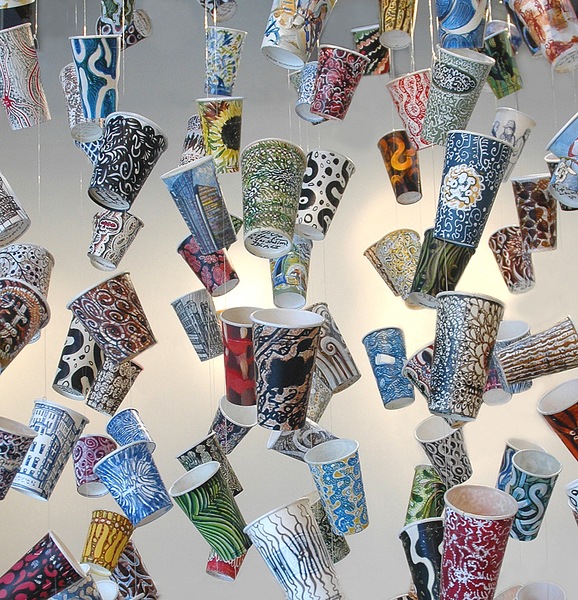
\includegraphics[width=\linewidth]{graphics/Gwyneth-Leech-cup5.jpg}
  \caption{Installation view}
  \label{fig:GwynethLeech_Installation}
\end{subfigure}
\hfill
\begin{subfigure}{.47\textwidth}
  \centering
  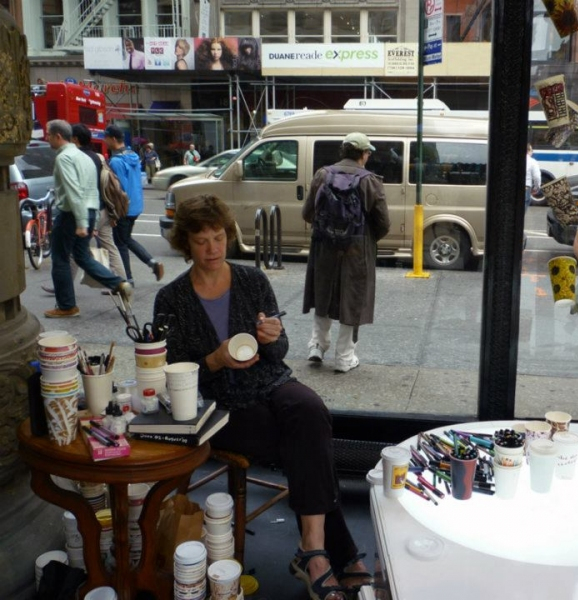
\includegraphics[width=\linewidth]{graphics/Gwyneth-Leech-cup3.jpg}
  \caption{Painting in the public}
  \label{fig:GwynethLeech_Public}
\end{subfigure}
\caption{Gwyneth Leech, 365 A Year in Cups, 2013, Mixed media on upcycled paper coffee cups, Dimensions variable}
\label{fig:GwynethLeech_CoffeeCups}
\end{figure}

I began to save all of my coffee cups to use as "canvases" for making art. Transforms coffee cups that are no longer trash but a vehicle for art, ideas, conversation and memories of a social moment upcycled from the detritus of our throw-away caffeine culture. I like my coffee or tea in a paper take-out cup. Even better than the contents, I like the used cup as a surface on which to draw and paint. And on the bottom of each one, I write the date, location, occasion and beverage consumed so that every hand-made cup artwork becomes the record of a social moment. Each cup representing a daily caffeine break. The installation makes visible largely unconscious patterns of consumption; this is what one simple take-away purchase looks like over the course of three years, this is what would usually be thrown away. It can be seen as a measure of time gone by, of money spent, of space to be taken up in a landfill. But as I upcycle each used cup into an artwork, it becomes the measure of other things as well: an artist's regular habit of generating new ideas, a diary of time spent with friends and colleagues, and the cumulative positive effect of doing something small and manageable every day. There are different versions of it. paintings on paper coffee cups displayed as installation in public window spaces. She publicly draw their cups (the cup art window installation and public drawing project were on view repeated showed at many places and date. During public drawing projects she draw with other people. and so. Buying a beverage is a daily event for Leech (and also many people. These coffee shops all around the world. As she drinks her coffee in the public, she also publicly transform its cup.


% TEA BAGS
% FROM https://instagram.com/silvirub/, http://www.rubysilvious.com/363-days-of-tea
\begin{figure}[h!]
  \centering
  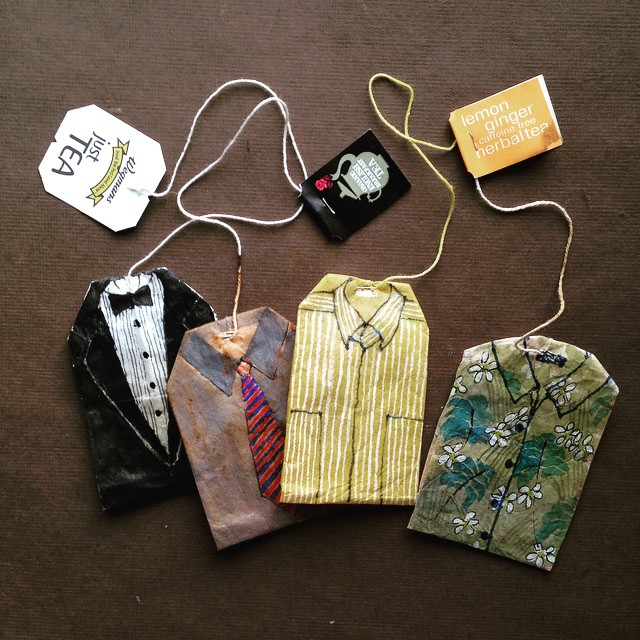
\includegraphics[height=6cm]{graphics/rubysilvious-teabag-Day169.jpg}
  \caption{Ruby Silvious, Day 169, 363 Days of Tea, 2015, Mixed media on upcycled paper tea bags, Dimensions variable}
  \label{fig:RubySilvious_TeaBag}
\end{figure}
  
Visual artist and graphic designer Ruby Silvious embarked on a quirky, personal experiment, set to last for 363 days. She decided to repurpose soggy and stained tea bags as unconventional, blank canvases, just waiting to be filled with her artistic expression. The project, entitled 363 Days of Tea, allows Silvious to challenge herself by transforming the recycled material with her intricate illustrations—the artist draws, paints, and forms collages on the salvaged tea bags. This project serves as Silvious’ daily journal, allowing her to record her thoughts and feelings by creating wonderful moody and whimsical designs on little teabag papers. Every day she creates a new piece that reflects her impressions in that moment. Currently based in New York, Silvious’ work has been exhibited internationally and she has received awards and recognition for her talents in paper work, print making and now her most recent endeavour of re-purposing recycled and found materials.


\begin{figure}[h!]
\centering
\begin{subfigure}{.47\textwidth}
  \centering
  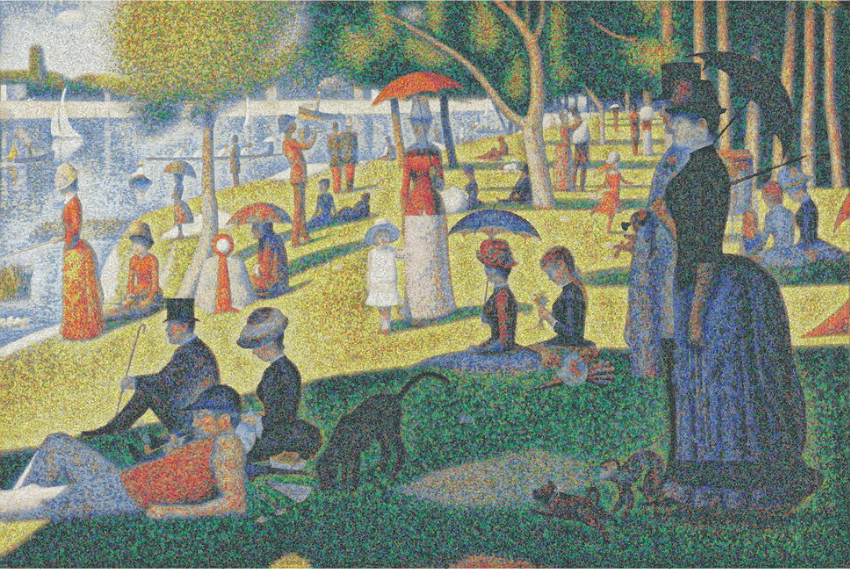
\includegraphics[width=\linewidth]{graphics/ChrisJordan_Numbers_OriginalView.jpg}
  \caption{Original view}
  \label{fig:ChrisJordan_Numbers_CloseView}
\end{subfigure}
\hfill
\begin{subfigure}{.47\textwidth}
  \centering
  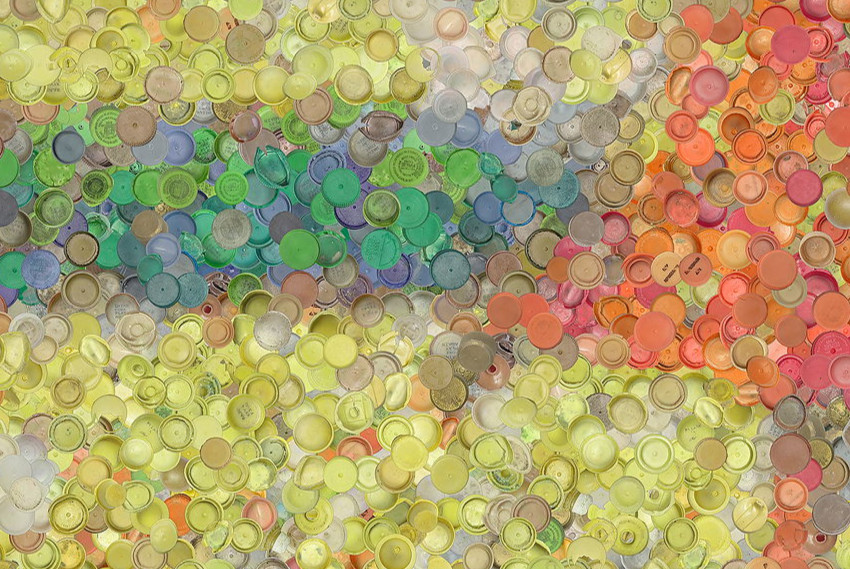
\includegraphics[width=\linewidth]{graphics/ChrisJordan_Numbers_CloseView.jpg}
  \caption{Close view}
  \label{fig:ChrisJordan_Numbers_OriginalView}
\end{subfigure}
\caption{Caps Seurat, 2011 60x90" in one panel, and 88x132" in 3 panels}
\label{fig:ChrisJordan_Numbers_CapsSeurat}
\end{figure}

Depicts 400,000 plastic bottle caps, equal to the average number of plastic bottles consumed in the United States every minute. Portraits of Global Mass culture from Chris Jordan. In Running the Numbers, photographer Chris Jordan attempts to convey the vastness of modern consumption by breaking down annual statistics into more graspable quantities depicted by clever visualizations made of individual objects or groups of objects that he photographs. “There’s a disconnect that happens when we assume we know what we’re talking about when we talk about hundreds of millions of plastic bottles,” Jordan says. “I’m trying to translate these numbers from the deadening language of statistics into a visual language that allows some kind of comprehension.” Many of Jordan's works are created from photographs of garbage and mass consumption Jordan uses everyday commonalities such as a plastic cup and defines the blind unawareness involved in American consumerism. His work, while often unsettling, is a bold message about unconscious behaviors in our everyday lives, leaving it to the viewer to draw conclusions about the inevitable consequences which will arise from our habits. He recreates the most remarkable artworks with combining bits of trashes as a mosaic. Here he draw attention to the our consumerism and express them numbers that are very big to understand. All the material that we have is trash to create this pictures.
\todo[inline]{Bu adam çok güzel bir şekilde küresel tüketimi ve onun sonuçlarını anlatıyor. Chris jordan hem bir gerçeği açığa çıkarıyor. Diğerinde ise belki de anlamamızı sor kılan gerçerkleri çöple ilgili, bizimle ilgili olanları gene bizim önümüze sunuyor. Bize konuya farklı bir açıdan bakmaya davet ediyor.}


%****************************************
% HAKAN GÜRSU
% Buraya aslında bir de Hakan Gürsu koymak gerekli olabilir. Yani aslında kendisi pek de sanatla ilgili bir laf etmiyor. Ama aslında tükettiğimiz onlarca şeye karşı bir tavır yaklaşım sergiliyor. Bu yüzden theory kısmında yer alabilir. Bu çöpün içinde boğulacağımızdan bahsediyor. Onu dönüştürmek gerekliliğinden yeteneğinden bahsediyor.


% TEZ STATEMENT.
% Ya gerçekten çöpü dönüştürüyorlar ya da çöpe dair düşünceleri dönüştürüyorlar, ve bunu ele alırken aslında heykel, kolaj, fotoğraf gibi şeylerden yararlanıyorlar ama aslında ortaya koydukları şey bir sanatsal eylem. veya bunu sanatsal eylem bağlamında ele alabiliriz.

% Aslında şöyle bir şey var mustafa, aslında sanatçının yaptığı şey ürünlerinden çok tekrar ve devamlı olarak eyleme geçirdiği yaklaşımı. Çöpün de bu tekrar eden yapısı buna uyum sağlıyor. Çünkü zaten hatayın sürekli bir parçası. Aslında bunun için şart olmasada destekleyici olduğu söylenebilir.

% Sanatçıların işlerine bir de bu açıdan baktığımızda ne görüyoruz.
%........................................

\comment{Things that are thrown away are one side of it. Actually all of our waste tells about us. ref required. Meaning of waste and what it tells about us. Understanding people through their wastes. REF. Tracey Emin's work. She opens up her wastes and also her life.}

% Related with tracy emin, photos of every cast off/discard/reject, understanding human through their discard.
\comment{GARBOLOGY} Garbology is a study of waste as a social science. Applying methodologies of archeology to the human debris. \todo[inline]{reference rubbish archeology of garbage} \paraphrase{"Weberman infamously used techniques of what he deemed garbology to uncover what he saw as the essential nature of people. He once said, perhaps indirectly referencing Jean Brillat-Savarin’s quote about food, “You are what you throw away.”" \cite{lukas2012garbage}}

% Garbology, from Encyclopedia, Abhijit Roy
\paraphrase{"The field of garbology involves the study of refuse and waste. It enables researchers to document information on the nature and changing patterns of modern refuse, hence assisting in the study of contemporary human society or culture. According to the Oxford English Dictionary, the term was first used by waste collectors in the 1960s. A. J. Weberman popularized the term in describing his study of Bob Dylan’s garbage in 1970. It was pioneered as an academic discipline by William Rathje at the University of Arizona in 1973."}\todo{ref.}

% Rubbish: The Archeology of Garbage, p.24
\paraphrase{As noted, the Garbage Project has now been sorting and evaluating garbage, with scientific rigor, for two decades. The Project has proved durable because its findings have supplied a fresh perspective on what we know---and what we think we know---about certain aspects of our life. (example of Medical researches)} \todo{ref.}

\begin{figure}[h!]
  \centering
  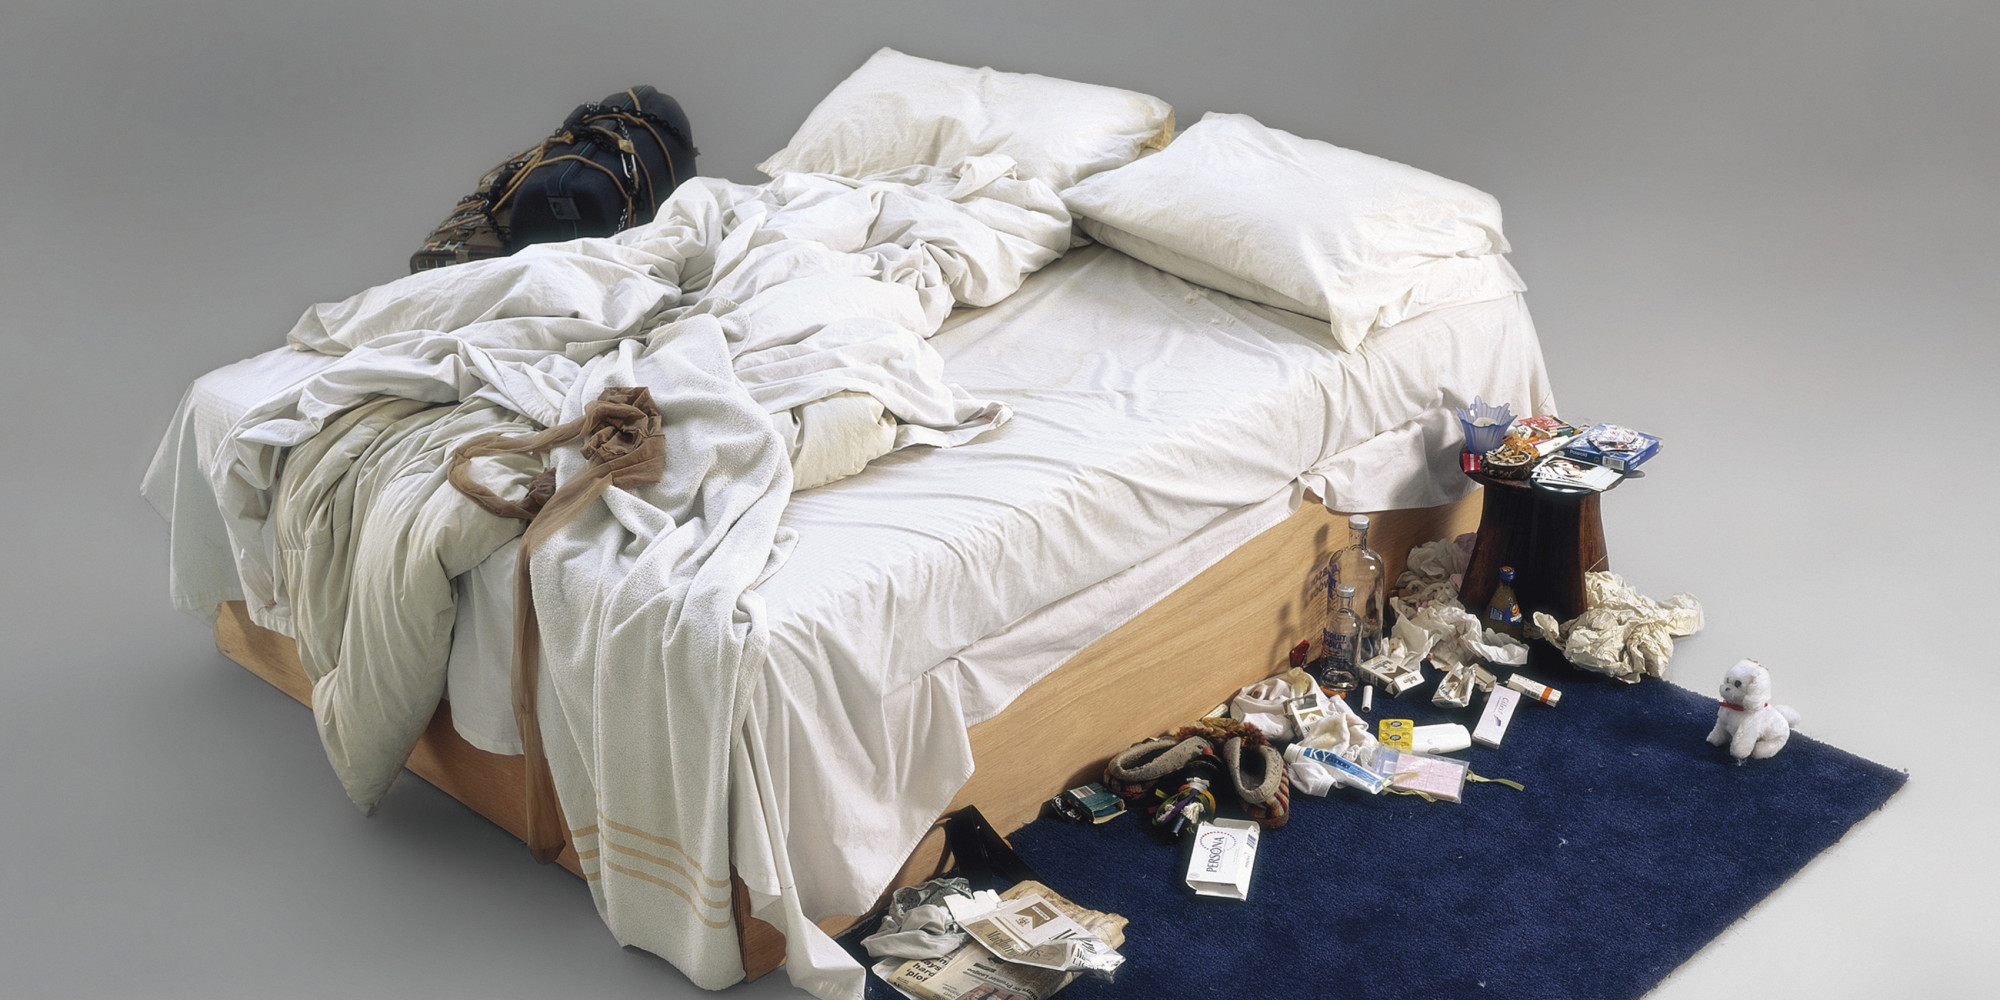
\includegraphics[height=6cm]{graphics/tracey-emin-my-bed.jpg}
  \caption{Tracey Emin, My Bed, 1998}
  \label{fig:TraceyEmin_MyBed}
\end{figure}

\paraphrase{Tracey Emin puts her private life to the public. The work, which Emin now describes as a portrait of a young woman. It is a time capsule. The cigarettes that litter the floor will one day no longer exist; neither will the newspapers. Around her there are pieces of junks speared all over the room. We can understand from her junk what type of life her has. We enter the world of artist through the her trashes.} \todo[inline]{Dört günden beri yataktan çıkmamış. İşte o sürede birikenler.}


%%%
%%%
%%%
% FROM Examined Life
\section{Zizek's Approach to Garbage}
(There is a curious fragment where Zizek, dressed as a sanitation man, stands in a waste deposit in a pile of garbage and ponders over garbage and human existence. In documentary film, Examined-life, Zizek talks about ecology in the middle of a garbage dump in London, and his part starts with these sentence: "This---garbage dump--- is where we should start feeling at home". He asserts his claim at first and go through explaining how ecology turns to ideology and mentions wrong perception about the ecology. Draw attention to notion of even if trash disappears from our world but not world. It seems as though the thrown out garbage disappears from our world. However, it disappears only from the world of illusions, but still exists in reality. He thinks that the way of approaching ecology is problematic, because accepting that nature as a balanced harmonious thing. He claims that it is ideological in the sense that wrong thinking important problems. Nature contains unimaginable catastrophes. think oil and distinct animals and plants. we profit balance part of the nature but it is created from catastrophe. Are we aware of this catastrophe. He asserts that ecology will slowly turn to religion that "is a kind of an unquestionable highest authority." Ideology of ecology warns us like, "Don't do that. It would be too much." its voice is like "Don't mess with D.N.A. Don't mess with nature. Don't do it" etc. We should not forget that we are part of the ecology. We must more alienated from the nature. We must find poetry and spirituality in the dimension of trash. That's the true love of world. Love is not about idealization. This part will be extended later.)

% FROM https://commons.wikimedia.org/wiki/File:Albatross_at_Midway_Atoll_Refuge_%288080507529%29.jpg
\begin{figure}[h!]
  \centering
  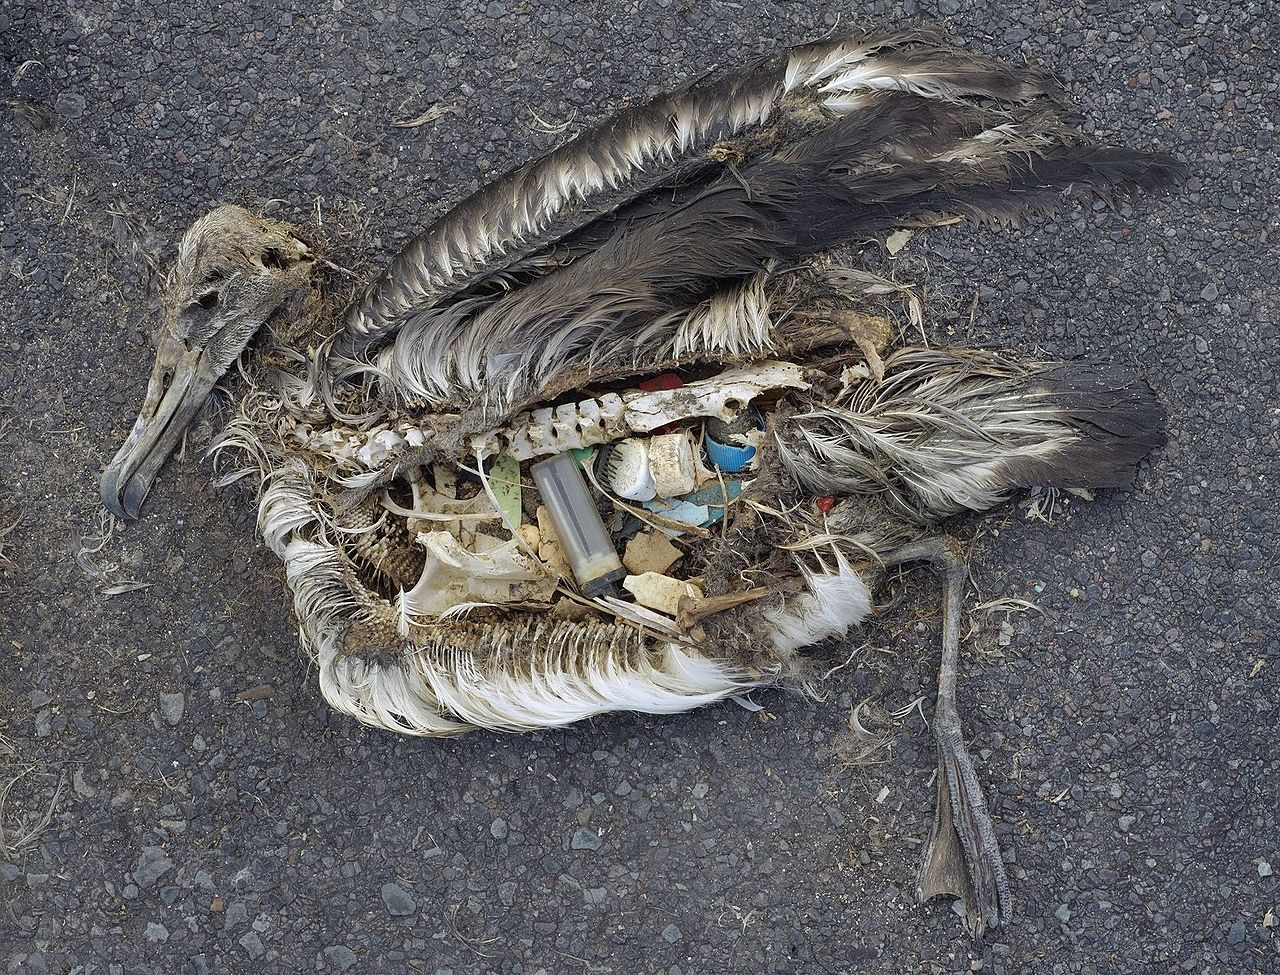
\includegraphics[height=6cm]{graphics/ChrisJordan-Albatross.jpg}
  \caption{Chris Jordan, Albatross at Midway Atoll Refuge, 2009}
  \label{fig:ChrisJordan_Albatross}
\end{figure}

The unaltered stomach contents of a dead albatross chick photographed on Midway Atoll National Wildlife Refuge in the Pacific in September 2009 include plastic marine debris fed the chick by its parents.

Using spare narration and stunning imagery, Chris Jordan's feature film MIDWAY explores the plight of Laysan albatross plagued by the ingestion of our plastic trash. Both elegy and warning, the film explores the interconnectedness of species, with the albatross on Midway as a mirror of our humanity.

Even if garbage leave outs our life, we do not care about the results of it. And it is captured by the works of Chris Jordan.In this photo series it captures 


% Effect of plastic on wildlife in Antartica.
% Her ne kadar biz çöpü attıktan bizim hayatımızdan çıksa da yok olmuyor. Sadece başka bir yerlere gidiyor. Mesela kuşların midelerine. Chris Jordan'ının imageları bunu çok da güzel açığa çıkartıyor. Bizim çöpleriminde habersiz hayvanlar bunları yiyorlar. Bir yandan ürettiğimiz ürünler ile kaynakları tüketirken bir diğer yandan ise artıklarımız diğer yaşanları tüketiyor. Dikkat çekmek istediğim nokta aslında ekolojik hassasiyetlerden çok aslında elimizde avucumuzda ne varsa onları tüketiyor olmamız. Karşı durduğum nokta ise tam olarak burası. 


\quotes{According to Zizek, modern understanding of ecology is the real false consciousness, connected with mystification of real problems. Postmodern mysticism arises when disasters begin to be rationalized, interpreted in strict logic terms of cause-effect relations. Such interpretation makes life easier. However, nature is not an absolute balance and total harmony (this aspect of Zizek’s thought makes him akin to classical conservatives). Nature is a series of unthinkable disasters. Zizek believes that ecology is transforming into a new western conservative ideology: “One should not play games with nature! Do not touch DNA! Do not develop new medicines! Do not invent new technologies!” How one should react to these reproaches? Zizek’s recipe is to reinforce alienation from nature, to become more artificial.} \cite{vafin2012zizek}

His basic argument is that the modern eco movement is a conservative ideology. It says don't do X from an authoritarian high ground and it idolizes and mystifies ecology. Basically he says the eco movement has it's head in the clouds. If it loved the environment it would recognize the rubbish we create and the chaotic nature of ecological change and try to further divorce itself from that process(nature) and try to turn the whole thing into art. 

\begin{itemize}
\item Our relation to our filth follows an “out of sight, out of mind” principle, but trash doesn’t disappear.
\item Ideology addresses real problems but mystifies them.
\item We search for meaning when a horrible event happens to make it easier to accept.
\item The ideology of ecology is that world is in the best possible state and that humans disturb nature.
\item Nature is not an organism in balance that humans exploit, but rather a series of great catastrophes.
\item Ecology is becoming more like religion with dogmas.
\item Even if we learn the potential catastrophes of nature, we ignore them as long as they don’t manifest near us.
\item The solution is not to worry about saving nature, but to figure out how to survive without it by becoming more artificial.
\item Learn to love our trash as a part of ecology.
\end{itemize}	

How much harmonious all these produced materials with nature? How many animals and the plant can use these discarded items? (Because of complex production methods their recycling requires complex processes again. Some of them already produced to protect goods from natural factors (like decaying etc.). However how can we protect nature from them?) It is very hard that spontaneously they become harmonious with nature. However, some artists turned to trash into site-specific sculptures that are more than trash heap. not discarding but bracing our attitudes turned them to a something that worth it to watch and think about it. (Converting what we create harmonious with the existing system.) Because it is not possible to think that nature will live harmoniously what we created. The more likely idea will be we will live harmoniously with what we create.

Getting rid of it is not the significant action. It still waits us at somewhere else or the next generations have to cope with it. (Establish relationship with the afterthought.) Maybe the first thing to do is accept the trash, to accept that there are things out there that serve nothing. To break out of this eternal cycle of functioning.

The issue of trash is not limited with ecological and economic perspective, it has also other dimensions.(draw attention to multidimensionality of this topic, but why? and what are the other dimensions?)

Trash itself is not the only problem, the practice, lifestyle causing it is more important problem. The dynamics of market and flow of objects into it plays important role production of trash.

Trash of developed societies has higher decomposing period in the nature. Therefore results in higher damage to the nature, hard to reuse, hard to transform, sometimes not to safe to keep them because toxic elements etc. 

\textbf{Summary.} Zizek mentions that ecology is something wrong point to approach this topic. Show the problematic understanding thought to the garbage. Suggest another thing, and point out the need for the new approach. Beyond the ecological problem there are different sides of it. Different readings can be added to the topic. Adding spirituality and new aesthetics dimension to the topic. 

% Her şey çöpe dönüyor. 
% En fazla ürettiğimiz şey çöp. Böyle giderse her şey her yer çöp olur mu? Aslında tezin konusu bu değil ve buna cevap verilmeyecektir? Ama WALL_E denilen dizi böyle bir alternatifte geçen bir dizi.
% İki tane yöntem var birisi bu çöp dağları... ve dağlardan ne görüleceği. Gerçi vik munizde o dağlara gidenlerden birisi ve oradaki insanlardan portreler yapıyor. Çöp dağlarını nasıl görmek gerek, nasıl farklı bir şekilde görebiliriz.
\comment{Zizekin çizdiği potreden aslında çöp dağlarınan oluşan bir dünya tasavvur edebiliriz. Ve bun noktada wall-e'ye bakabiliriz. Bir an için çöpümüzün içinde buğulacağımızı düşünürüz. Ya da bu çöp dağlarının bizleri sınırladığını düşünebiliriz.}

%\comment{WALL-E belki olabilir. Dünyanın aslında bir çöp yığını haline gelmesini gösteriyor olabilir. Çöp dağları, çöp denizleri. Atılmış binbir türlü nesne. ve wall-e ise bunları ne yapıyor sadece pressleyip bir kenera bırakıyor. Bundan basetmişken aslında pressleme işi yapan şu cesar. Bu şekilde olmak zorunda mı? Bunun alternatifi yok mu? Aslında bu tezde bunlara cevap bulunabilir. Çöpe olan bir sürü yaklaşıma ek olarak bir de bunlar var. Ya da başka neler var? Bunları araştıran inceleyen bir yazı. Wall-E'nin çizdiği portreyi tekrar ele alırsak ne görürürüz. İnsanlık buna mı dönüşücek? Başka bir ihtimal yok mu? Gerçekten de dünyayı bekleyen şey bu mu? Bir çöp yığını olması mı? Bu bir abartı mı yoksa gerçeklik payı yadsınacak cinsten mi?}

%\comment{WALL-E is a 2008 American computer-animated science fiction comedy film produced by Pixar Animation Studios. A robot named WALL-E, who is designed to clean up an abandoned, waste-covered Earth far in the future. WALL-E resembles giant dozers that moves and piles trash in the landfills. This robot creates squeezed trash blocks that have no meaning and interpretation. All different objects in terms of their physical and social properties turned to same squeezed garbage blocks. There are mountains of trash and place is very limited. By squeezing them, WALL-E saves space. \todo{What is the context of it? Which part is related with my topic?} What are we going to do with all these mountains of trash? \todo{Can it be placed under zizek part?} WALL-E represents a possible future condition of Earth.}

% HERŞEY ÇÖPE DÖNÜYOR. Relationship between entropy (second law of thermodynamics) and waste. Resources of nature turns to waste that it can revert it. Creating that are reversible again is problematic through the nature of sustainability. What is produced after it is consumed become worthless.

% Yani bir çözüm bulmaktan bahsediliyor ama sanat çözüm bulur mu bilmiyorum. Zaten derdim de benim aslında tüm bu çöp sorununu ele almak çözmek değil. Çöpe olan bakış açısındaki problemi göstermek olabilir. Burda beni destekleyen şey zizekin sözleri olacak.

idealization of nature, to love nature is to love trash. Live with trash. Do not see it as trash actually. Then the question is how to love trash? how to live with trash? can living with our trash enrich (our perceptions, abilities)? how not to see them as trash and useless? Can it be possible with art?

%%%
%%%
%%%
\section{Rubbish Theory}
Objects have a lifetime and they don't remain same through that lifetime. Their value, usage, location change over time. During its lifetime objects may circulate different markets and values systems like economical value, social value, aesthetic value etc. Especially this cycle has picked up speed with the advent of consumer culture, our most recent technological gadgets becoming obsolete within 3 years. Objects function and value are transformed by relocation and revaluation of objects from one place to the other or one discipline to another. This flow(transition) and transformation theorized with Rubbish Theory by Thompson \cite{thompson1979rubbish}. Thompson looks at the creation and destruction of value in man-made objects, cultural artifacts, and ideas. He notes how an object’s economic and/or cultural value diminishes over time rendering the objects worthless or redundant. The theory looks at how some of these objects then regain value, such as antiques or historic homes. It claims that there are three types of objects; transient (normal state, decreasing value, circulating), durable (permanent, increasing value, removed from circulation) and rubbish(zero value, will be destroyed or reinvested for economic and social value). The transition from transient to durable is only possible firstly transient to rubbish and later rubbish to durable. Further, there is a common idea/argument/motto that is "trash to treasure" among artists who use trash as a medium. Rubbish theory presents a conceptual approach to this argument. 

Although Thompson is quite successful categorizing states of objects throughout their lifetime, claimed transitions between states in the theory have some problems. Thompson label some transitions as possible and the others as impossible. "He allows goods only to move from a transient to become rubbish, and from rubbish they can either be destroyed or become durable. Movement in the other direction, from durable to either transient or rubbish, is not allowed in this system" \cite{meadow2011relocation}. Further, he does not allow move from transient to durable. However, Duchamp's fountain breaks this rule. Because urine used as a fountain is still functional and have a place in the market. In another word, it is not rubbish. This urine with the approach of Duchamp turned to be an artwork. It is one of the most influential piece of modern art and one of the best examples of ready-made. After Duchamp's intervention to the urine, it becomes a durable object placed in a museum.

In rubbish theory beyond the objects states how it happens transition of objects in practice is missing and Parsons fills this gap by claiming that transition from rubbish to durable are possible with finding objects, displaying objects, re-using objects \cite{parsons2008thompsons}. (explain details) (It can also be thought that they are the way of value creation.) (turning trash to treasure or something else is a value problem. transforming them creates new a value system? or just finding place existing value system. by the way there is a value theory related with (or inside of) game theory.)

Further another conducted research examines the psychological, social, and aesthetic factors involved in found object and found that ... \cite{camic2010trashed}.

"Rubbish theory, a philosophy that attempts to address how value is placed on material objects." "It is a body of thought that addresses how the value of material objects is socially constructed and deconstructed." "An awareness of rubbish theory is important to the understanding of the sociology of consumption and waste because, while what is and is not considered garbage may seem obvious and natural, the value of objects is based on the perceptions of people." "The classic examples of these categories are the durable 18th century Queen Anne tall-boy chest and the transient used automobile." "What decides whether or not something is a durable or transient is often the perceptions of the powerful members of society, those with a vested interest in owning objects whose value will always increase, while the remainder of society owns objects whose value will eventually decrease to nothing."

The paper suggests the Theory is useful in foregrounding the material dimensions of markets. It also highlights the importance of thinking in terms of movement, flow and circulation in markets. Finally the theory suggests that value emerges through our ways of seeing and placing objects. (From Liz Parsons)

%%
%%
\subsection{Rubbish Theory in Practice}
% TODO PRAP. REF.
(Summary From Liz Parsons.) 

A key critique of the rubbish theory is its neglect of the practices of value creation. Thus the paper draws from existing studies in consumer research in exploring three such sets of practices: finding objects, displaying objects, and transforming and re-using objects.

Plenty of work in consumer research explores the ways in which goods might act as symbolic resources for lifestyle and identity construction (i.e. Belk 1988), but there is less reflection on the actual practices and activities through which goods become meaningful and valued. McCracken’s (1988) work on ‘Meaning Manufacture and Movement in the World of Goods’ begins to address this gap. He views advertising and the fashion system as instruments of meaning transfer between the culturally constituted world and consumer goods. He then suggests that a series of consumer rituals operate to transfer meanings from consumer goods to the individual consumer. These rituals include those of possession, exchange, grooming and divestment. The strengths of his argument include a focus on the mobile quality of meaning and some exploration of the instruments though which meaning is transferred. However he is not clear as to the practices which constitute these rituals. In addition his contention that ‘meaning resides in three locations: the culturally constituted world, the consumer good, and the individual consumer’ (1988: 89) fails to completely capture the complexity and fluidity of meaning movement. There is a linearity to his conceptualisation which misses the constant flux and flow of meanings in markets.

In ‘The Social Life of Things’ Appadurai (1986) highlights the restlessness of objects arguing that ‘from a methodological point of view it is things-in-motion that illuminate their human and social context.’ (1986: 5). Appadurai usefully observes that ‘commodities, like persons, have social lives’ (1986: 3). He focuses on the ‘commodity potential’ of things. ‘things can move in and out of the commodity state, that such movements can be slow or fast, reversible or terminal, normative or deviant’ (1986: 13). However these movements do appear to be reduced to the opposites of commoditization and singularization, one might ask the question, does anything exist in-between? This is where Thompson’s Rubbish Theory comes in.

\subsubsection{Transients, Rubbish and Durables}
The category of objects and experiences of no value (rubbish objects and experiences) is largely invisible. The transient represents the usual state of commodities as objects which are declining in value and which have finite life spans. Whereas the durable increase in value over time and have (ideally) infinite life spans (1979: 7). Thompson uses the example of a used car as a transient and Queen Anne tallboy as a durable. He further observes that their category membership determines the way we act towards them. 

Thompson argues that rubbish represents an important possible ‘in-between’ category in a ‘region of flexibility’ which is not subject to the same control mechanisms of the valuable and socially significant categories of transient and durable. Therefore it ‘is able to provide the path for the seemingly impossible transfer of an object from transience to durability’ (1979: 9) he further suggests that ‘a transient object gradually declining in value and in expected life-span may slide across into rubbish’ (1979: 9) where it has the chance of being re-discovered, brought to light or cherished once gain. Figure one demonstrates the possible paths an object may take (from transient to rubbish and from rubbish to durable). 

Thompson comments that we only notice rubbish when it is in the wrong place, and highlights the embarrassment and anxiety that mis-placed rubbish, or rubbish which has found its way in to the wrong place can cause ‘Something which has been discarded, but never threatens to intrude, does not worry us at all.’ (1979: 92) but rubbish in the wrong place is ‘emphatically visible and extremely embarrassing’ (1972: 92). (Further there is similar analogy at Waste and Want. The author give the example of shoe and claim that thrash is relative. The shoe on the dinner table is something disgusting but in the foots is not at like that.) Rubbish objects are things that are no longer used or loved or cared for and often no longer seen. Rubbish objects linger on the periphery of our lives, in the back of the drawer, bottom of the wardrobe or cupboard, corner of the garage or garden shed gathering dust.

\quotes{In an ideal world\ldots an object would reach zero value and zero expected life-span at the same instant, and then... disappear into dust. But, in reality, it usually does not do this; it just continues to exist in a timeless and valueless limbo, where, at some later date (if it has not by that time turned, or been made, into dust) it has the chance of being discovered’ (1979: 8-9)}

\subsubsection{The Practices: From Rubbish to Durable}
Three such sets of practices are explored below, they include: finding objects, displaying objects and transforming and re-using objects. It is argued that each of these sets of practices changes the way we view an object moving it from being seen as a ‘rubbish object’ of no value to a ‘durable object’ of increasing value.

\textbf{Finding Objects:} One key way in which objects may slide from the category of rubbish to durable is through the act of finding. Indeed, Gabriel and Lang (1995) include the ‘Consumer as Explorer’ as one of many possible consumer identities.What, then might one mean by ‘the find’? Ultimately the find relates to discovery, and suggests that something has been otherwise overlooked, ignored or hidden away. The find may not involve objects which are new to us, it is possible to find some of ones own items if they have been hidden away long enough in an attic and thus made strange to us. The concept of the find also suggests that the found object has some qualities that others (or indeed ourselves) have in the past overlooked, as such it is closely related to ‘bringing to light’. The find may be extended to embrace features of objects as well as objects themselves. This directs us to their ‘potentialities’, objects may have been there all along but we’ve suddenly found them to be useful, likeable or beautiful. It might be that some aspect of them has simply been brought to our attention. Equally, as discussed below in relation to transforming objects, we may make alterations to objects which bring out their potential. The transition from thing of little or no value (rubbish), to thing of value (durable) can result form a relatively minor shift in the way we see something.

\textbf{Displaying Objects:} by displaying objects in home, fashion etc. (This is not a strong category.) Maybe publicly exhibiting them. 

\textbf{Transforming and Re-using Objects:} These transformations may involve creating new uses for old things to fit in with contemporary lifestyles. Transformations may also involve the modification or updating of objects through painting, alteration or repair. Transformations may not only be based around creating new uses but also creating new looks. The re-use of objects also creates value for things that otherwise would be allowed to slip away (or slide terminally into the rubbish category).

%%
%%
\subsection{Theoretical Analysis of Found Object}
(Summary From Paul M Camic.) 

% TODO PRAP. REF.
\subsubsection{Seeking Objects}
As a species Homo sapiens has been gathering and collecting objects for thousands of years. Food, clothing, weapons, fuel, animals, and plants are the more obvious items, but visually pleasing objects, things that arouse curiosity, and shapes that stimulate the imagination have also been sought. The search for “things,” collecting them (Humphrey, 1979), and the need to embellish and make the ordinary special (Dissanayake, 1988) have been essential parts of the evolutionary process of human development (Bettinger, 1991; Dissanayake, 1992). For example, many early cave drawings occur around a natural feature within the cave such as a projection or indentation (Bahn, 1998; Lewis-Williams, 2004), making these natural features potentially comparable to found objects in modern and contemporary art (Read, 1930). When early prehistoric eople recognized a cave’s natural feature as a “found object” and incorporated it in a picture, it is possible that the natural feature took on a higher value than if left alone, thus adding to the value of the object on the cave wall. Once found and incorporated in paintings and drawings on a cave wall, it is possible that these protrusions and indentations became objects that functioned symbolically.

In contemporary societies, people seek objects to adorn bodies, decorate homes and gardens, and personalize places of work (Menzel, 1994). Seeking and finding objects, whether in vast Asian cities, remote African villages, or the high streets of Europe and North America, have become part of daily life for millions of people. Although most of these objects are purchased new in shops or online, many others are preused items, castoffs, or trash found in back alleys and country lanes, dumpsters, and rubbish bins or purchased cheaply in flea markets, garage and boot sales, and in shops catering in previously owned goods. Some individuals have chosen to salvage objects out of economic necessity, as depicted in Jean-Francois Millet’s 1857 painting The Gleaners and by Agne`s Verga’s 2002 documentary film Les Glaneurs et la glaneuse, whereas others have done it for a range of other reasons, including a desire to rescue them (Belk, Wallendorf, \& Sherry, 1989). These “other reasons” pose an opportunity for researchers to better understand why people voluntarily seek society’s discarded material objects and how they make use of them. A form of cultural reuse, the process
of salvaging and using found and second-hand objects has potential implications for \ldots 

% [TODO adapt for my case] The main aim of the current study was to produce an initial conceptual model that explains contemporary found and second-hand object use in blablabla.

% [TODO adapt for my case] Found objects first came to the attention of the general public through their use by artists in early part of the 20th century. To help contextualize the application of found objects, the following section provides an overview of their use by Western artists. This is followed by an examination of objects in human development and includes aspects of psychoanalytic theory, material objects and their relationship to identity, selected cognitive theories, and an outline of the social life of objects through rubbish theory.

% Amelie olabilir. Orada fotoğraf toplayan çocuk olabilir. Onları itinayla toplayan bir adam. Tren garındaki fotoğraf kulubesi. Belki de dünyanın dört bir yanından gelen insanlar, bir kesişim noktası. Bir birinden farklı bir sürü insan. Filmde neden böyle bir eyleme yer veriliyor? Film fotoğraflar üzerinden defter üzerinden ilerliyor. Onun çevresinden bir hikaye kurgulanıyor. İnsanların artıklarını topluyor. Onların değer vermedikleri şeyleri topluyor. Bunlar baya baya aslında o insanlar. Bazı fotoğraflar çok fazla küçük parçalara ayrılıyor. Çok iyi bir örnek mi bilmiyorum. Burada niyet nedir ki? Ben buna şöyle bir okuma getireceğim diyebilirim. Amelie mesela küçük ayrıntılara dikkat eden bir insan, bu fotoğraf taplama işi de aynı şekilde. Bu arada bu fotoğraf toplama işi ilk değil. Found photos diye başka bir paper var ve orada aslında bu işin ilk uygulaması gösterilmekte. Ama benim işime yarayan kısmı ne? Neden o fotoğrafları ya da bunun filmini yapıyor. Aslında puzzlelar üretiyor. Belirli tekrar olacaktır. insanların kapalı bir ortamda nasıl pozlar verdiklerini sonrasında ise onları attıkları şeylerden görülebilir. Tekrar bir kitap haline geliyor. Tanınmayan insanların fotoğrafları. Nerde oldukları, neden ve nasıl çekildikleri belli olmayan bu yüzden aslında ilişkilerin insanlara bırakıldığı bir koleksiyon. Aslında tam da amelie bunu yapmıyor mu? Hikayeler üretiyor bu fotoğraflardan. Yeni karşılaşmalar üretmesi. Her ne kadar sıradan portre fotoğraflar olsa da birbirlerinden oldukça farklılardır. Bin bir türlü şey vardır aralarında. Nereye yerleşmeli. Başkasının çöpünü toplama. O dönemin o eşyasını arşivini tutma. ve herkes sunuluyor sonrasında bu.

\subsubsection{Found Objects in Art}
The term found object, as used in this article, refers to an existing object or artifact that is picked up (found) and generally not bought or originally intended as art, yet it is also considered to have some value (e.g., aesthetic, novelty, remembrance) to the finder. It is during the locating and finding process that the value of the object, once considered to be junk or rubbish, changes. The junk object becomes transformed into the valued found object. Objet trouve, translated from the French as “object found,” appears to have been first used by Marcel Duchamp in 1913 in reference to objects he made use of in his “readymade” art (Richter, 1965). His earliest known application for an objet trouve was seen in his well-known piece Bicycle Wheel, “where he had simply upturned a wheel on a stool” (Gale, 1997, p. 97) and labeled it a work of art. A more public and controversial introduction of the readymade occurred in 1917 when Duchamp attempted but failed to exhibit the highly contentious piece The Fountain, where a single white urinal became a readymade piece of art (Tomkins, 1996). These pieces were the beginning of Duchamp’s shift from an art striving for beauty and possessing a higher complex or hidden meaning beyond what was seen to an art form that made use of, and occasionally celebrated, the common materials and objects found in everyday living.

Gascoygne (1936), writing about the artist’s use of “the strange medley of materials” (p. 169), referred to as objets trouve in Surrealist art, suggesting that the artist “discovers a hidden symbolic significance in the [found] object which is preserved when the object is ‘framed’ as art” (p. 170). The finder discovers an unrealised significance in the object. A new boundary is formed around the object by the finder through removing it from its found environment and placing it in a new one, thus empowering the finder in the role of creating a new reality for the object. He argued that the found object, before it is found, approximates a zero value aesthetically; the zero value increases for the finder---beholder on discovery of the object and increases further if the object is placed in another context. \ldots the meaning of material objects was derived from their symbolic relation to another (e.g., person, time, place, experience) rather than through their physical attributes (Causey, 2003; Csikszentmihalyi \& Rochberg-Halton, 1981). 

How a region of flexibility develops, what social factors are involved in taking innovative and creative responses toward rubbish, and how an individual changes (and enhances) his or her creative responses toward society’s detritus are areas that require additional examination. (Important points a gap in the literature. Although Parsons article analyze practices, it is not very broad and detailed. Further what is the importance of it is missing.)

Camic's \quotes{project surveyed participants who currently use found objects in their daily lives in order to investigate and understand possible purposes, determining factors, and potential benefits of their use.} 

\todo[inline]{table moved to drafts.}

The importance and enjoyment of found objects to those who participated in this study, using them in various ways and for different reasons, were strongly evident. The interaction between finder and object is an attempt to make meaning of an object that has been found, and by being found and desired becomes transformed.

Gascoygne (1936) recognized that finding an unrealized significance in a material (found) object was empowering partially because, through the creative agency of the finder, the object’s aesthetic value had increased from zero to something greater. The transformation of rubbish from a negative value to a positive value requires the finder to develop a symbolic meaning, and sometimes a functional use, for the object that goes beyond its present situation as culturally labeled detritus while simultaneously responding to its current physical and aesthetic elements. When the found object is seen by the finder as a symbol representing another entity (e.g., when an old blue bottle with foreign lettering comes to symbolize far away intrigue, mystery, and sophistication), support is given to what Dittmar (1992) described as socially constructing a material identity for the object. Expanding on Dittmar’s use of a social interactionist perspective, the results of the present study support the possibility that the entire found object process---finding, reclassifying, and reusing objects---becomes a symbol of identity for the finder. This supports Digby’s (2006) argument that individuals make use of salvaged objects as souvenirs, which are no longer part of the commodity cycle, to rework and construct individual and social identities.

An important difference, however, which also appears to contribute to the aesthetic experience, takes place when discovering an object unexpectedly in a nonpredetermined place and time. Unlike appreciating art in a museum, which is a boundaried activity occurring at a scheduled time and place with the anticipation of finding and looking at art objects, finding discarded objects can occur anywhere at anytime and thus, according to participants, can “trigger” a burst of sensory attention and a “surge” of cognitive activity on the part of the finder. 

Results of this study also support consideration of found objects as important artifacts that are signifier of cultural meaning.


%%%
%%%
%%%
\section{Summary}
\begin{itemize}
\item Moving nature of trash/objects.
\item Classification is the main key, trash is not related with the object property. 
\item Value creation, shifts in the society. 
\item Trash has archaeological value.
\item Trash has potential to be used again.
\end{itemize}

Thompson thinks that the switch only occurs from losing all the value given the object. He refers that to gain new value previous systems ruins must be cleaned. Changing the context by first rubbishing them.

Thompson and Zubiaurre say trash moves between value states, Zizek says you must love your trash and bricolage can be the name of this practice.

Firstly trash is created (by the throw away culture). Even if there is counter argument about it, the focus is disposable items and their amount is very high. After generating mountains of garbage the approach of zizek introduced. What to do this garbage see. He claims that we need to find a way to handle it. Find aesthetics and other things. Learn to live with the trash.

% Burada zizekten rubbish theorye geçerken aslında bir bağlantı bulmalı. İkisi arasında bir ilişki kurmalı. Ya da aslında static değildir çöp arkadaş bak bunu ileriki kısımda rubbish theory ile sana anlatacağım diyeceğim  mesela. 

Later rubbish theory and relative approach to the trash. Trash is not static. Objects are not static. It related with the perception. Classification of them. It is possible to change shift. Practices of it.

% Aslında burda bazı pratikler veriliyor. Ama daha detaylısı bir sonraki bölümde verilecek. Sanat bağlamına yoğunlaşılarak. 

Then next chapter discusses the practices in art world in more detail. Trash in the context of art. Which purpose and which method? Approaches of artist.

% Bu bölümün faydası ne oldu bana. Neleri çıkartmış oldum. Tüm bunlara göz atmak gerekli.
% - ilk olarak throw away culture denilen bir şey var. belli çeşit üretim ve tüketim yöntemleri var. ve sanatçılar bunu karşı eleştirel yaklaşmışlar. hatta bir şeyin alternatifi olduğunu söylerken bunun neyin alternetifi olduğunu göstermem gerektiği için kullanıyorum. Konu çok geniş olabilir. kapitalizm, endüstrileşme faktörler olabilir. Aslında ben bu kültürün nasıl oluştuğundan değil nasıl şeyler ürettiğiyle ilgileniyorum. Büyük çöp yığınları oluşturuyorlar. (Benim kimin çöpüyle uğraşıyorum. Yani aslında bir sürü çöp var. Biraz da bunu netleştirmek için buna ihtiyaç var.)

% - Sonrasında ise bu çöp yığınlarını ne yapacağız. Dert bu. Nasıl yaklaşmak gerekli bu çöp yığınlarına. Burada belki bir kaç yaklaşım verilebilir. Ama ben zizekin yaklaşımını ele alıyorum. Çünkü adam demiş ki çöpünüzle birlikte yaşayın. Ben de zaten bunu yapmaya çalışıyorum işimde. 

% - Çöp ile birlikte yaşa diyorsun ama bu nasıl olacak. en azından mümkün mü? Burada aslında çöp dediğin şeyin aslında bir şeyin bir sınıflandırma sorunu olduğu ve farklı stateler arasında geçişler yaptığını görebiliriz. Çöp evlere değinmek gerekebilir.

% Sonra bu iş pratikte nasıl oluyor ona bakılabilir. 

% Yeri gelmişken pisuvarı da bu rubbish theorynin sınıflandırmasına sokabilirim. 

Zizek points out wrong opinion about ecology among the society.

\chapter{Trash (in) Art}

\epigraph{One day, in a rubbish heap, I found an old bicycle seat lying beside a rusted handlebar, and my mind instantly linked them together. I assembled these two objects, which everyone then recognized as a bull’s head. The metamorphosis was accomplished, and I wish another metamorphosis would occur in the reverse sense. If my bull’s head were thrown in a junk heap, perhaps one day some boy would say, \quotes{Here’s something that would make a good handlebar for my bicycle!}}{\hfill ---Pablo Picasso, \textit{Trashformations}}


Its roots go all the way back to the 1800s in Europe.

How and why does trash draw attention of artists(, and also mine)? In this chapter how artist approached to the trash and their techniques are discussed in the context of art. (Historical development, methodologies, tactics, motivations\ldots) Focused on visual (plastic) arts(, because there is also a music genre called as trash music?). How does it turn to medium?

% TODO List motivations of artists and their ideas about junk. Because it reveals the different dimensions of this topic.

% Diğer tezlerde ne diyordu. Bu nasıl bir anlatış biçimi be mustafa. doğru düzgün bir şey yok. Anlatcak olsan birisine böyle mi anlatırsın ha?

%%%
%%%
%%%
\section{Root in the Art History}
In this chapter root of using ---(non-art)--- objects in the artworks is examined. In other words using objects in artworks beyond their intended purpose or intended meaning and function. Developing artworks not only painting but also using paper and other stuff by pasting them together. (Foundations of trash in art.) Using object apart from their proposed meaning is not a new thing[ref required, using jewelry by African tribes], through the ages people used objects and tools for different purposes. However it is not discussed in the context of (western)art and not accepted method for art making. Therefore who and which work introduces this concept and how it is developed and evolved in time. (of course it is a brief overview by some remarkable pieces.)

% TODO paraphrase
\quotes{The use of trash as a fine art medium dates back at least to the work of early-20th-century artists such as Fortunato Depero and Kurt Schwitters. Use of found materials, including garbage, has been associated with assemblage art since the 1950s and has been practiced by other well-known artists, including graphic artist Christian Boltanski, sculptor Louise Bourgeois, and photographer Andres Serrano. Art made from garbage has since become much more common in fine arts venues such as museums, galleries, and high-profile installations, including H. A. Schuldt’s famous “Trash People,” which has traveled around the world since 1996}  \cite{tauxe2012encyclopedia}.

\todo[inline]{örnek bulduğum tezlerin izlediği yolu burda izleyebilirim.}

%****************************************
% FROM The Ruin and the Ruined in the Work of Kurt Schwitters by Gemma Carroll
% The German avant-garde was working from ruins literally and metaphorically, and trash was both practically and freely available; to use it was an action that took the ruins of our society, its discarded, to question how meaning is constructed.
% Marx wrote that it was not the materiality of the object but the social relations that create value, the use of urban detritus in particular, the squalid results of mass-produced human relations, infuses the materiality of Schwitters’ work with an anthropological quality.
% Karl Marx had already written that economic value does not inhere in the materiality of the object but emerges from the social relations and organisation of labour which produces it, and that the separation between consumer market and the sphere of culture had become indiscernible.
% Schwitters is able to use the ruined, the waste products, as an anthropological exploration of society from both its unpleasant outcomes and its decay. \ldots trash was both practically and freely available; to use it was an action that took the ruins of our society, its discarded, to question how meaning is constructed. As he wrote: ‘It grows more or less according to the principle of a metropolis.’ 13 The Merzbau was itself a city; and just as Marx wrote that it was not the materiality of the object but the social relations that create value, the use of urban detritus in particular, the squalid results of mass-produced human relations, infuses the materiality of Schwitters’ work with an anthropological quality. Material has transformed into information, and ‘how’ has surpassed ‘what’ we see. The grottos in the Merzbau that still reveal this detritus most clearly could not be re-created in Bissegger’s reconstruction because, arguably, they are an exploration of absence, an exploration of ruin. As Schwitters wrote: ‘One can even shout out through refuse.’ 14 His words still echo.
%........................................

%%
%%
\subsection{Collage}
Collage originates from the French \textit{coller} is an artistic technique of applying manufactured, printed, or “found” materials, such as bits of newspaper, fabric, wallpaper, etc., to a panel or canvas, frequently in combination with painting. In about 1912–13 Pablo Picasso and Georges Braque extended this technique, combining fragments of paper, wood, linoleum, and newspapers with oil paint on canvas to form compositions. Pasting paper is not a new technique but using this it in the art making is a revolutionary movement in the  language of art \cite{waldman1992collage}.

% Works of picasso baraque.

% TODO reading...
\cite{greenberg1984collage}

%%
%%
\subsection{Assemblage}
Assemblage work produced by the incorporation of everyday objects into a composition. It is similar to collage, but main difference is that assemblage is three dimensional rather collage is two-dimensional. Diverse range of things can be used production of work. In 1961, the exhibition "The Art of Assemblage" was featured at the New York Museum of Modern Art. William C Seitz, the curator of the exhibition, described assemblages as being made up of preformed natural or manufactured materials, objects, or fragments not intended as art materials \cite{seitz1961art}.

\todo{Joseph Cornell, assemblage artist.}

%%
%%
\subsection{Bricolage}
Dictionary meaning; something constructed using whatever was available at the time.

% daha öncesinde birbiri ile bağlantılı olmayan nesne, söylem, metin, form, pratik vs. gibi şeyleri yeni bağlamlarda yeni anlamlar üretmek için montajlama, yap-boz edimi;

% ingilizcesi do-it-yourself anlamına gelen fransızca bir kelime. bunu yapan kişiye de bricoleur deniyormuş. lévi-strauss'un kitapları ingilizce'ye çevrilirken diy/craftsman tam olarak anlamı karşılayamadığından çevirilerde de bricolage olarak kalması tercih edilmiş. kendi başına da anlamlı olan öğelerin yeni bir bağlam çerçevesinde birleştirilmesi ve bu parçalardan yeni hikayeler, efsaneler yaratılması edimine de entelektüel brikolaj diyebiliyormuşuz.

Claude Levi-Strauss notes: the bricoleur works not from the principle of making things only if natural resources are available but makes things according to those things at hand, making do with what is available. It is an expression that, like the natural cycles of the Earth, attempts to make something new from something old. \cite{levi1966savage}

the “bricoleur” is \ldots someone who works with his [or her] hands and uses devious means compared to those of a craftsman \ldots \cite{levi1966savage}

\begin{quote}
[He or she] is adept at performing a large number of diverse tasks; but, unlike the engineer, he [or she] does not subordinate each of them to the availability of raw materials and tools conceived and procured for the purpose of the project. His [or her] universe of instruments is closed and the rules of his [or her] game are always to make do with “whatever is at hand,” that is to say with a set of tools and materials which is always finite and is also heterogeneous because what it contains bears no relation to the current project, or indeed to any particular project, but is the contingent result of all the occasions there have been to renew or enrich the stock or to maintain it with the remains of previous constructions or destructions.\cite{levi1966savage}
\end{quote}

\ldots someone that creates bricolage is described as a \quotes{bricoleur, an odd-job man who works with his hands, employing the bricoles, the scraps or odds and ends}. 

\begin{quote}
The bricoleur, says Levi-Strauss, is someone who uses 'the means at hand,' that is, the instruments he finds at his disposition around him, those which are already there, which had not been especially conceived with an eye to the operation for which they are to be used and to which one tries by trial and error to adapt them, not hesitating to change them whenever it appears necessary, or to try several of them at once, even if their form and their origin are heterogenous---and so forth. There is therefore a critique of language in the form of bricolage, and it has even been said that bricolage is critical language itself\ldots If one calls bricolage the necessity of borrowing one's concepts from the text of a heritage which is more or less coherent or ruined, it must be said that every discourse is bricoleur.\cite{derrida1993structure}
\end{quote}

\begin{quote}
The engineer, whom Lévi-Strauss opposes to the bricoleur, should be the one to construct the totality of his language, syntax, and lexicon. In this sense the engineer is a myth. A subject who would supposedly be the absolute origin of his own discourse and would supposedly construct it 'out of nothing,' 'out of whole cloth,' would be the center of the verbe, the verbe itself. The notion of the engineer who had supposedly broken with all forms of bricolage is therefore a theological idea; and since Lévi-Strauss tells us elsewhere that bricolage is mythopoetic, the odds are that the engineer is a myth produced by the bricoleur.\cite{derrida1993structure}
\end{quote}

% TODO reading...
[TODO use this ref]\cite{strasser1999waste}

Bricolage is different than collage. Bricolage > collage. Because it is more general understanding of human practice. Collage is just only gluing paper together and it can be only a subset of bricolage. Same applicable for assemblage. Transforming trash can be examined within bricolage. 


%%
%%
\subsection{Found Object (Ready-mades)}
Found object originates from the French \textit{objet trouvé}, describing art created from undisguised, but often modified, objects or products that are not normally considered art, often because they already have a non-art function. Pablo Picasso first publicly utilized the idea when he pasted a printed image of chair caning onto his painting titled Still Life with Chair Caning (1912). Marcel Duchamp is thought to have perfected the concept several years later when he made a series of ready-mades, consisting of completely unaltered everyday objects selected by Duchamp and designated as art. The most famous example is Fountain (1917), a standard urinal purchased from a hardware store and displayed on a pedestal, resting on its side.

% Duchamp falan.

\todo[inline]{place in the folk art.}

%%
%% junkyard art
\subsection{Garbage Art, Recycling Art}
"Garbage art (alternatively known as trash art or recycled art) is art created from materials including post-consumer and other waste, collected debris, or objects previously used for other purposes." "Creating art from garbage involves transforming the meaning of objects by placing them in new, aestheticized contexts. This practice is not new; tribal peoples have adapted bits of trash from industrialized societies into their traditional arts since coming into contact with products of the developed world." "Creating art from trash involves “consuming” garbage in the sense that artists appropriate and rearrange the materials in personal ways, transform their meanings, utilize them to their own ends, and represent them in new ways.It involves taking unwanted materials out of their “waste” context and recontextualizing them as “art.”" \cite{tauxe2012encyclopedia}

% TODO From Beautiful Trash Art and Transformation BY PAOLA IBARRA, ReVista
Recycling has always been a common practice in the arts at least at a non-material level. From creating a world of words in literature, to rhythm and images in poetry, sampling in hip hop music, representation in the visual arts, or editing the illusory continuity of a film, art implies taking disparate elements (ideas, images, references, objects, etc.) and putting them together to form a new whole. Take and put. De-contextualize and re-contextualize. In that sense, art, as a system, is an act of recycling [from PAOLA IBARRA].


%%%
%%%
%%%
\section{The case of \quotes{The Gleaners and I}}
The Gleaners and I is a 2000 French documentary film by Agnès Varda that features various kinds of gleaning. The Gleaners and I is notable for its fragmented and free-form nature along with it being the first time Varda used digital cameras. This style of film making is often interpreted as a statement that great things like art can still be created through scraps, yet modern economies encourage people to only use the finest product.

It's a self-reflexive film because the director establish a relationship with the practice of gleaners and her film making practice. Some people gleans crops, the others discarded food, the other baby dolls and Agnès Varda gleans images.  

\quotes{Agnès Varda’s film, The Gleaners and I, documents the history and current practice of gleaning in France. Historically, gleaning is the act of collecting leftover crops from farmers’ fields after the harvest. However, in the film Varda expands this definition to include actions that are presently coined \quotes{dumpster diving} where people collect any types of rubbish or unwanted items to reuse them in their own way. Moreover, Varda includes her actions of collecting images with a video camera as gleaning. She is gleaning images. The Gleaners and I far more than document the lives of gleaners. It highlights the degree of global consumerism of the modern world and the ways art can exist within it in relation to gleaning.}

The official subject of this film is gleaning, the act of gathering remnants of crops from a field after the harvest. As Varda demonstrates, people can be discovered throughout the French countryside gleaning everything from potatoes to grapes, apples to oysters, much as they did hundreds of years ago (though no longer in organized groups). More figuratively, there are also urban gleaners who salvage scraps from bins, appliances from the side of the road, or vegetables from stalls after the markets have closed. And then there’s Varda herself, a gleaner of images, driving around France with a digital camera and a tiny crew (at times, she wields a smaller camera herself, permitting an even greater degree of intimacy).

Making use out of something that has been left behind and labeled as obsolete is not unique to farms and crops. There is so much discarded, yet still-viable food in dumpsters that many people live off it entirely. Seeing the value in what someone else has defined as trash is an art in itself.

Once as a common practice of gleaning throughout the years has evolved, but not disappeared. She keeps light to the modern life gleaners that are not visible every time. One of the interesting thing is here Agnès Varda feels that as a aging person will later become discarded person. In other word we can be subject of the refusal. At some point she become the subject of the thing that she track. 

There are many aspects of this documentary film. First draw attention the practice of gleaning. The discarded items that are not fit in the industrial standards because of their shape, color etc. Even if these items are discarded and we are not aware of them, there is also another life for them. Modern life gleaners feed from them. In another words someones trash becomes another trash. There are people live the boundaries of consumption societies. They create their life from the unwanted items. what the society refuses, they find a life or create a life from them. Their lifestyle is also can be seen as alternative to the life on the urban areas with deep relationship with the consumerism. (as also Zizek mentions that love is not idealization. But the industrial processes has some standards and beyond that standards there is not a place for everyone. Life is being lived in the cites is somehow idealized life or tried to be idealized life. beyond the border of the urban there is new life generated. What is not succeed in the cities succeed outside of it.)

She uses unconsciously recorded pieces in the film. \quotes{The last definition of gleaning, gleaning images, ties into what I found both the most amusing and perplexing scene in the film. It is the scene where Varda had forgotten to turn her camera off and accidentally films the ground and her lens cap bouncing along as she walks. She sets this scene to a jazz soundtrack. While watching the scene I was certainly confused. Why is this in here? What does this have to do with gleaning? And certainly why did the scene last so long? But there was also something lovely about it. Maybe it was the music, but for some reasons my senses found it audibly and aesthetically pleasing. I wasn’t able to make much sense out of the meaning behind this scene; I believe Varda referred to it as \quotes{the dance of the lens cap}.  Luckily, Ruth Cruickshank’s article, The Work of Art in the Age of Global Consumption: Agnes Varda’s Les Glaneurs et la glaneuse (The Gleaners and I), addressed this scene and clarified the potential deeper meaning behind it. Cruickshank likened the scene to something that is normally thrown away, or in this case edited out of the film, much like the way trash is thrown away or food is left behind after a harvest. Varda gleans the image of the dancing lens cap, \quotes{Where many documentary makers would leave such accidental footage on the cutting room floor, Varda draws attention to how what would habitually be perceived as waste may be viewed as supplement with its own intrinsic value. Rather than literally treating it like dirt, Varda retains and prompts reassessment of that which is normally left out of shot} \cite{cruickshank2007work}. Things that are often forgotten or discarded can easily be revamped to create something useful to someone. The scene was revamped using music and it became beautiful, much like the gleaners who found fish in the trash cooked it to make it edible, or the artist gleaner who piled discarded baby dolls into totem poles.} 

Refused is not only foods and trash. there are a lot of things that are pushed outside border of the society. She talks and investigates artist that are using discarded items in the artworks. What people not found anything the artist see countless possibilities from them. There is always alternative ways to see something different. Giving life or finding life from discarded life.

The clock found the garbage pile and taken by Agnès Varda. It does not work properly but it has important meaning for her. The time does not go on and it does not remind her that she is aging.

Here another point is that Agnes display images of people picking up things from the ground like their ancestors. Everyone somehow collecting things in their life but particularly she selects these people and their images in action. There should reason for this? For some individuals, gleaning is not a novelty or a clever way to save money, but a necessity of life. They require it to sustain their life. Combine the elements from different peoples that seems totally unrelated gains powerful theme for the documentary. What gleaning means become more open (or powerful). It draws a picture of body combination of different parts (connected, dependent to the each other). The reason of gleaning varies but the fact that gleaning is continues in different forms.

She discusses the importance found in the meaning and purpose of art forms like this: \quotes{Varda seeks to encourage viewers to consider what potential agency is demonstrated in the artfulness and contingency of gleaning by individuals excluded\ldots from the homogenizing systems of global consumption} \cite{cruickshank2007work}. One can find more treasure in trash than many of New York’s finest galleries and art exhibits; they bring a grassroots feel to what has always been seen as a stuffy and prude aspect of society.

The Gleaners And I is not an environmental film. Gleaning, Varda implies, can be understood more broadly as a form of resistance, a way of refusing to be boxed in by conventional expectations; as such, it demands that we re-learn age-old skills as well as supply individual creativity and initiative.

The film tracks a series of gleaners as they hunt for food, knicknacks, thrown away items, and personal connection. Varda travels the French countryside as well as the city to find and film not only field gleaners, but also urban gleaners and those connected to gleaners, including a wealthy restaurant owner whose ancestors were gleaners. The film spends time capturing the many aspects of gleaning and the many people who glean to survive. One such person is the teacher named Alain, an urban gleaner with a master's degree who teaches French to immigrants.

Varda's other subjects include artists who incorporate recycled materials into their work, symbols she discovers during her filming (including a clock without hands and a heart-shaped potato), and the French laws regarding gleaning versus abandoned property. Varda also spends time with Louis Pons, who explains how junk is a "cluster of possibilities." Louis Pons (born 1927) is a French collage artist. He specializes in reliefs and assemblages made entirely from discarded objects and junk. In Agnès Varda's documentary The Gleaners and I, Pons explains his artistic process and understanding of art; what others see as "a cluster of junk," he sees as "a cluster of possibilities;" and that the function of art is to tidy up one's inner and exterior worlds.

%%%
%%%
%%%
\section{Examples from contemporary artists}
Artist and artworks related with trash and their analysis. Stages of their works and methods. (Keep in mind that what can be extracted from these works?) There are a lot of work that needs to mentioned here but to stay focused and not to move away from the scope of the thesis only the works are selected with relation to the theory chapter. (is it really like that?) 

% FROM ReVista
Trash is dirty. Trash is smelly. Trash can provide the raw materials for exquisite art---from sculpture to film and beyond.

% FROM Paola Ibarra ReVista
Whether in sculpture, photography or other media, art frequently deals, directly or by allusion, with daily challenges of life in Latin America and elsewhere. Is there a limit to recycling and representation? Or is there a point at which waste cannot become art (or anything else)?

% TODO Naive debate??
All that can be seen as naive act because of little impact and outside of the system(which system?). As it compared to the huge portion of the material the transformed material is so little therefore it can be questioned that it has no impact and worthless as it compared to the mountains of landfill. However this very argumentative that having no impact or little impact. It might be true that this practices solve all problems of landfill or etc. But changes individuals and communities life. It recreate and rebuilds the community. Even if it is one simple object worth look and see the opportunities of it. 

\begin{itemize}
% FROM Maite Zubiaurre, Re Vista Garbage
\item \textbf{Road Kill.} Filomena Cruz creates photographic series “Road Kill” painstakingly captures tiny “trash corpses” on the pavement. It is that particular type of trash meet in the public places. trash left behind, trash on the sidewalk, squished, squashed, and weathered. Filomena Cruz sees trash that we don’t want to see. A piece of chewing gum with an “engraved” leaf; a flattened-out tube; a corroding paper napkin with a still intact heart; or a frog-green Crayola melting in the heat, all speak the language of “worthlessness” suddenly becoming meaningful (and moving).For one thing, trash corpses faithfully record city life. 

% They are continuously changing. Unrecognized things. Created unintentionally. Part of the streets roads. It can be seen as a archive.

  \begin{figure}[ht]
      \centering
      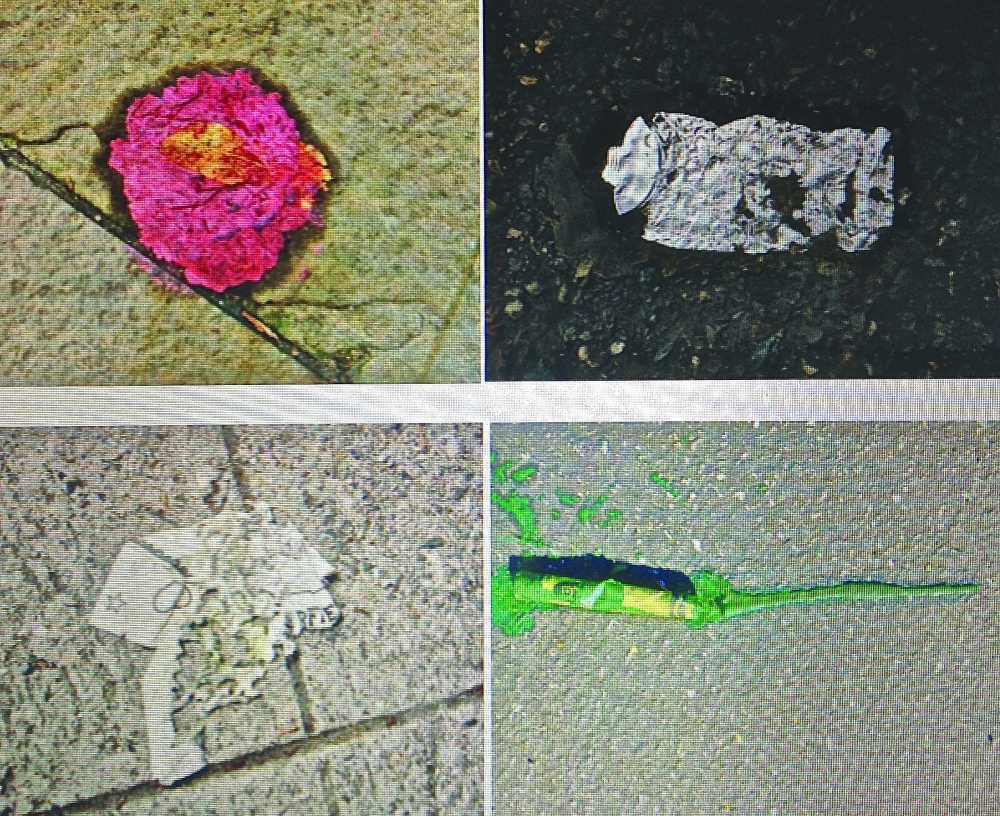
\includegraphics[width=0.8\textwidth]{graphics/FilomenaCruz_RoadKill_ReVista.jpg}
      \caption{Road Kill by Filomena Cruz}
      \label{fig:FilomenaCruz_RoadKill_ReVista}
  \end{figure}

%\item Pictures of Garbage by Vic Muniz
\item \textbf{Pictures of Garbage.} Vic Muniz creates monumental trash art in Jardim Gramacho with the help of \textit{catadores} (Waste Land, 2010) Waste Land, directed by Lucy Walker  tracks the development of a series of monumental photographic portraits made from trash. Called “Pictures of Garbage,” they were created by Mr. Muniz in collaboration with the garbage pickers of Jardim Gramacho, an open-air dump just outside Rio that is one of the largest landfills in Latin America. (Important point is here collaboration with the pickers. Listening their stories and capturing their portraits. What is specific about trash here?)

% Talking with people picks up trash. Goes to landfill?

  \begin{figure}[ht]
      \centering
      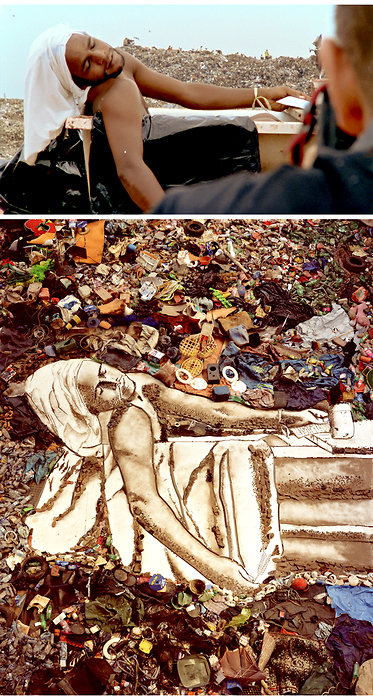
\includegraphics[width=0.5\textwidth]{graphics/vik-muniz-picturesofgarbage0.jpg}
      \caption{Pictures of Garbage by Vic Muniz}
      \label{fig:VicMuniz_PicturesOfGarbage}
  \end{figure}

\item \textbf{The Recycled Orchestra.} Favio Chávez and Nicolás Gómez decide to build musical instruments out of garbage and get 35 children from Cateura, Paraguay’s biggest trash dump, to travel the world with their “Recycled Orchestra”. ``The world send us garbage. We send back music''.

Cateura, Paraguay is a small city that has grown atop a massive dump. It is regarded as one of the poorest slums in Latin America, a village where people live among a sea of garbage. Incredibly, the landfill itself is the primary form of subsistence for many residents, who pick through waste for items that can be used or sold. Prospects for most of the children born in Cateura is bleak as gangs and drugs await many of them. But then one day, something amazing happened. A garbage picker named Nicolás Gómez (known as “Cola”) found a piece of trash that resembled a violin and brought it to musician Favio Chávez. Using other objects collected from the dump, the pair constructed a functional violin in a place where a real violin is worth more a house. Using items gleaned completely from the dump, the pair then built a cello, a flute, a drum, and suddenly had a wild idea: could a children’s orchestra be born in one of the most depressed areas in the world? As you can guess, the answer was yes.

To view scenes from the landfill slum of Cateura in Paraguay is to look into the depths of extreme poverty. But within the contents of the landfill are glimmers of hope in the form of cardboard, utensils and other discarded materials that can be crafted into imperfect but usable musical instruments. These makeshift violins, flutes and cellos, combined with instruction from a local music teacher, have given birth to the Recycled Orchestra of Cateura. Through the music of Mozart, Beethoven and Vivaldi, this orchestra allows the young musicians to transcend their identity as children of poverty.

"A violin is worth more than a house here," says Favio Chavez, the orchestra's director and founder. In the midst of such an existence, these musicians have created something both special and truly awe-inspiring. "My life would be worthless without music." says one girl in pigtails. A young man named Juan Manuel Chavez, nicknamed Bebi, has a cello fashioned out of an oil can and old cooking tools. For the camera, he plays the Prelude to Bach's Cello Suite No. 1 — beautifully.

"People realize that we shouldn't throw away trash carelessly," says Chavez at the end of the trailer. "Well, we shouldn't throw away people either."

This project can be seen as a bricolage practice. They build their musical instruments from what is available around. 

\begin{figure}
    \centering
    \begin{subfigure}[b]{0.45\textwidth}
        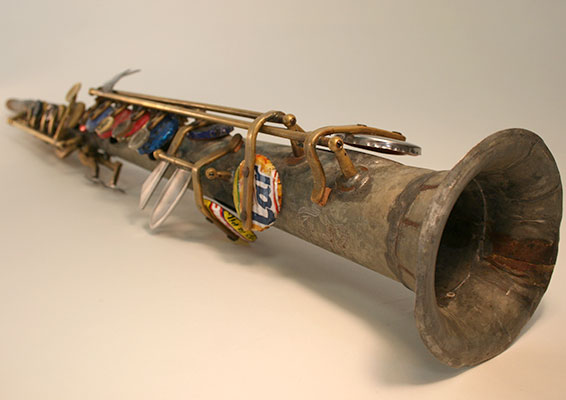
\includegraphics[width=\textwidth]{graphics/landfill_harmonic-sax.jpg}
        \caption{Sax}
        \label{fig:landfill_harmonic-sax}
    \end{subfigure}
    \begin{subfigure}[b]{0.45\textwidth}
        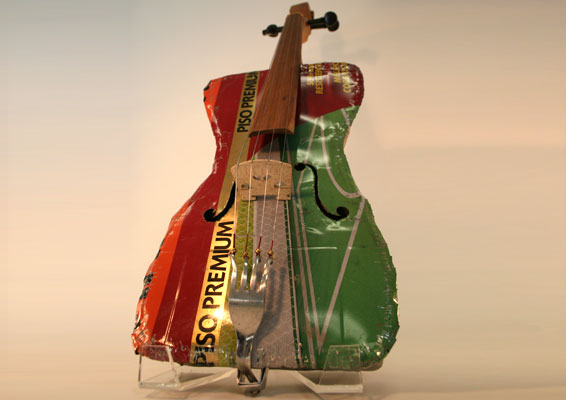
\includegraphics[width=\textwidth]{graphics/landfill_harmonic-violin.jpg}
        \caption{Violin}
        \label{fig:landfill_harmonic-violin}
    \end{subfigure}
    \caption{Instruments of Recycled Orchestra}\label{fig:animals}
\end{figure}

% Dönüşümün aslında burada görebiliyorsun. Yav bu sanat mı peki? Sadece maddelerin dönüşmesi değil onlarla birlikte insanlarında dönüştüğünü görebiliyorsun burada. 
% Beni bu projede etkileyen en önemli şeyler: ilk olarak oradaki insanların hayatlarını değiştirmesi, hiç hayal edemiyecekleri bir noktaya ulaşmaları, tümünüde kendi emek ve yetenekleriyle başarmaları. yokluk içinden bir şeyler üretmeleri. Her ne kadar üretilen müzik aletleri mükemmel olmasalarda onlar için bulunmayacak bir nimet. Üretilen ürünün kalitesi gerçekten de endüstriyel standartların altında. Müziğin kalitesi diğer kadar olmasa bile farklı bir yaklaşım sunuyor olması önemli. Nasıl oluyor da bu aletten bu ses çıkıyor. Amatör ruhun getirdiği bambaşka bir algı var. Müziğin ötesi, düşündürdüğü bambaşka şeyler var, olaya yeni bir boyut getiriyor. Başka bir alanla diğerinin buluştuğunun bir göstergesi.

% Peki bu iş neden sanat işi olsun ki? 

% Bambaşka şeylere dönüşen ürünler. Üretim amaçlarının dışında. Yeni linkler bağlantılar kuran müzik aletleri. Kendilerinden beklenmeyeni başarmak vs. Daha önce görülmeyen şeyler, görülmeyen ilişkiler.

% Bunu bir okuyabilirsin.
% http://www.publicbooks.org/interviews/recycling-literary-culture-a-conversation-with-lucia-rosa
% http://www.eloisacartonera.com.ar/ENGversion.html
\item “Eloísa Cartonera,” a work cooperative in Buenos Aires, proudly produces handmade books with cardboard covers: \quotes{We purchase [\ldots] cardboard from the
urban pickers (\textit{cartoneros}) who pick it from the streets. Our books are on Latin American literature, the most beautiful we had a chance to read in our lives.} \quotes{Some of them are preserved as art books at university libraries, while others circulate as literary pieces expected to disintegrate in time---something anticipated of the material they are made from.} [from PAOLA IBARRA, ReVista]

It reminds me that litreary is also a reuse concept. Because to create meanings we reuse words and idioms again again with different combination. \comment{tüm kelimeler vs hepsi sıralanıyor. Arka arkaya getiriliyor. Kelimeler harflerin hepsi tekrar tekrar kullanılıyor. Reused cartbord reminds all of these and as an object all of it...}

\todo[inline]{Bu ne anlama geliyor onu bulmak gerekli. nereye bağlamalı bilemiyorum. Bu ileri dağıtmak gerekiyor ama gene de burada kalanlar var. Ne yapsam ki?}

  \begin{figure}[ht]
      \centering
      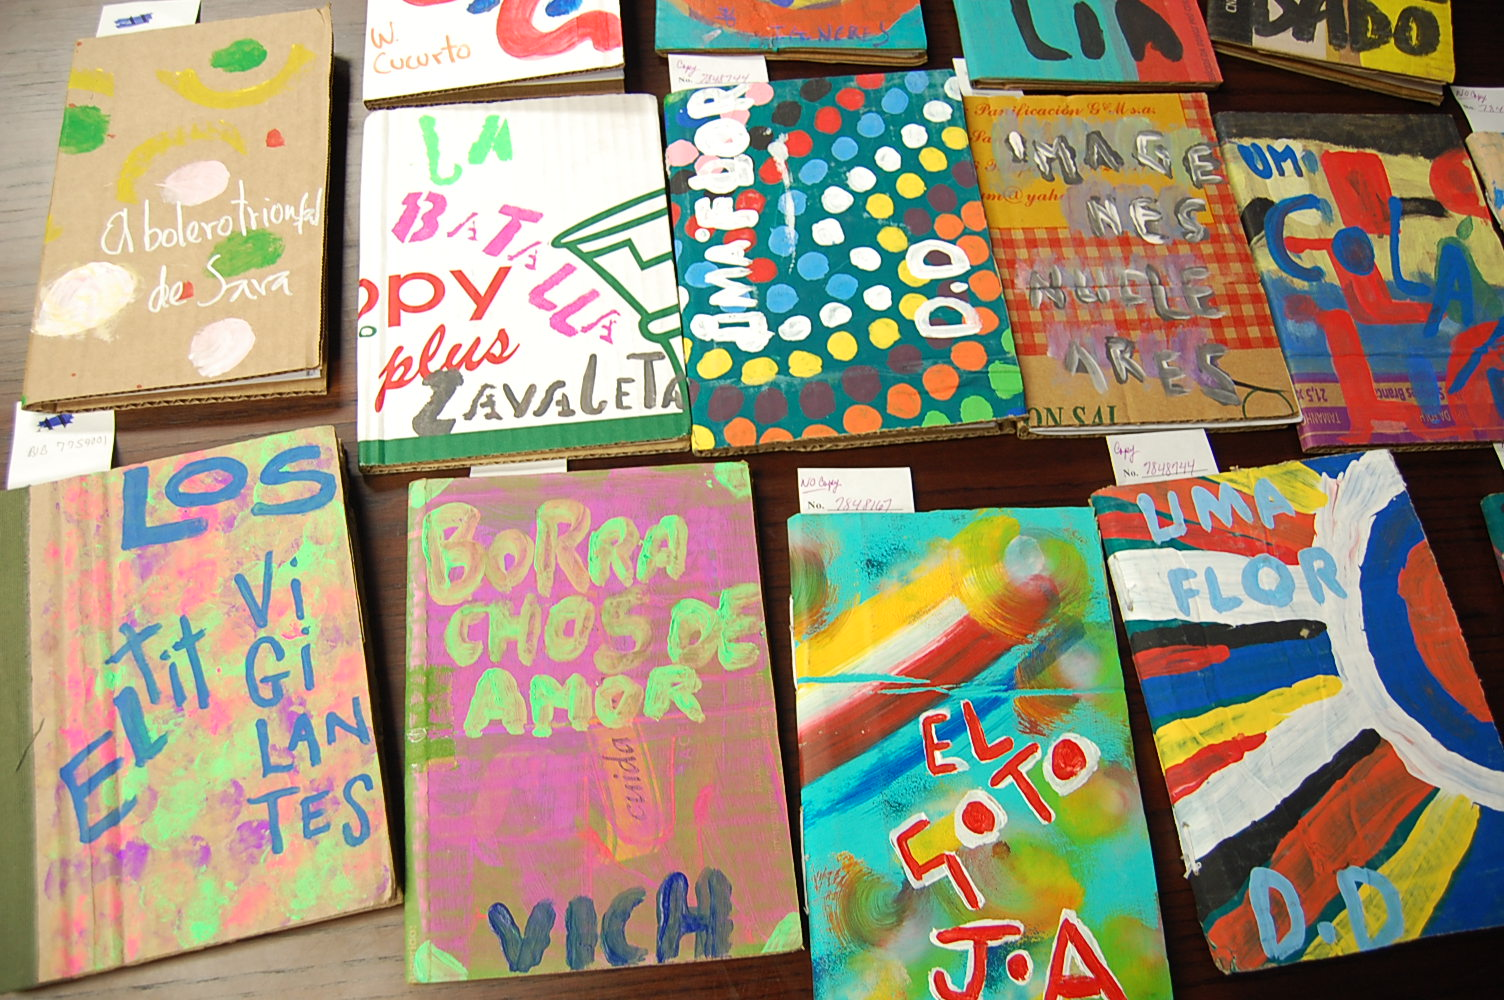
\includegraphics[height=6cm]{graphics/EloisaCartonera_Books2.jpg}
      \caption{Books covered by Eloisa Cartonera}
      \label{fig:EloisaCartonera_Books}
  \end{figure}

% FROM Paola Ibarra, ReVista
%\item Forever; Blue Yonder by artist Kyle Huffman
%\item Too Too---Much Much by Thomas Hirschhorn
%\item Autoconstrucción by Abraham Cruzvillegas

% Bu adamın ilkeleri var. Benim de var aslında.
% FROM A Present from the Sea BY SONIA CABANILLAS, ReVista
% https://www.youtube.com/watch?v=v6IoEF_Tsrw
%\item Nick Quijano has some rules to create assemblages. \quotes{There are certain self-imposed rules to this creative process: first, the assemblages or artefactos must all come from material washed ashore on this beach; second, it must be plastic and industrial refuse, result of the processing of fossil fuel; third, it must be polished by a long stay in deep waters, sometimes even encrusted with corals, shells or pebbles, or simply scraped by the ocean floor. As a sign of respect and sacralization, these pieces will be incorporated without any adjustment: no cutting or bending, seen as a mutilation of the object. Its identity cannot be veiled or masked but always must be recognizable amidst the other components; e.g, a comb must remain a comb even as one may see it as a mustache.} The sea returns this refuse; it is not biodegradable.

% FROM Burning Messages BY MICHAEL WELLEN, ReVista
%\item Antonio Berni

% FROM Haiti in the Time of Trash BY LINDA KHACHADURIAN, ReVista
\item Haiti case. When I ask him why he chooses to work in the medium of trash, he replies, \quotes{It gives respect to my city to use the garbage. It shows that everything can be used, and nothing was lost.} (TODO motivation: \quotes{I get more inspiration working with recycled materials because those pieces are unique and can’t be duplicated}) Eugène says that he’s partial to metal, which has become more and more difficult to find because of the clean-up initiative by the city. When I ask him if part of him wishes there were no such effort underway, he answers: \quotes{No. When you have clean streets you have good health, and that is the most important thing.} (This is very strange. It shows that working with trash and being clean healthy is not a contradiction. Both of them exist together.) \quotes{Other people come to Haiti and see junkyards, but we see magical playgrounds,} Jean explains as he watches them.

% FROM Thinking on Film and Trash BY ERNESTO LIVON-GROSMAN, ReVista
% By the 1950s a film like Tire Dié (Fernando Birri, Argentina, 1956) already portrays the collecting, classifying and recycling of trash not only as a source of informal income but as a commercial activity linked to the formal economy. In these films, trash is not the end of a process of consumption but the beginning of a cycle of production. These movies share the idea that trash could be a departure point to think about the modern condition as defined by consumption, class disparities, contamination and urban development. The poet Charles Baudelaire is one of the first to make the connection between the rag picker and the modern city. Walter Benjamin picks it up and from then on the fragmentary condition of trash will remain associated with contemporary art and ultimately with the Modern condition: the industrial refuse could be redeemed by art. It is in this sense that filmmaking becomes allegorical and mimics the process of recycling when it reappropiates archival materials and found footage to create new narratives from scraps, fragments, of films that were not in any way connected to these new narratives.

\item \textbf{American Beauty.} The film American Beauty , which features a long, poetic clip of a plastic bag swirling on an eddy of air, snagged five Academy Awards, yet I for one still find it hard to think of plastic bags as things of beauty. 

% Recycled art.
%\item \textbf{Aaron Kramer.} His motto: "Trash is the failure of imagination." \cite{meyer2007turning} In addition to concern for the environment, Kramer was drawn to recycled art because of one simple factor---the price. "Free is certainly great, and that was a driving force for me early on in my career," he said.

% http://www.tate.org.uk/art/artworks/nelson-the-coral-reef-t12859/text-summary
\item Nelson’s breakthrough work was The Coral Reef, which he mounted in 2000 at Matt’s Gallery from objects and debris gathered from alleys, trash bins, and car-trunk sales all over London. The title refers to Nelson’s aim of creating an intricate, reeflike network of lives “all existing under one sea, which is capitalism,” he says. (It is very corralate between Ages Varda's work. She shows at the side of human practice, Nelson looks the topic from object side.)

\todo[inline]{very important maybe the second case will this one.}

% From http://www.thisiscolossal.com/2014/06/historical-fine-oil-portraits-on-crumpled-trash-by-kim-alsbrooks/, http://www.thisiscolossal.com/2015/05/new-historical-portraits-on-flattened-cans-by-kim-alsbrooks/, http://kimalsbrookswhitetrash.blogspot.com.tr/
\item
\parbox[t]{
	\dimexpr\textwidth-\leftmargin}{%
      \vspace{-2.5mm}
      \begin{wrapfigure}[22]{r}{0.4\textwidth}
        \centering
        \vspace{-\baselineskip}
        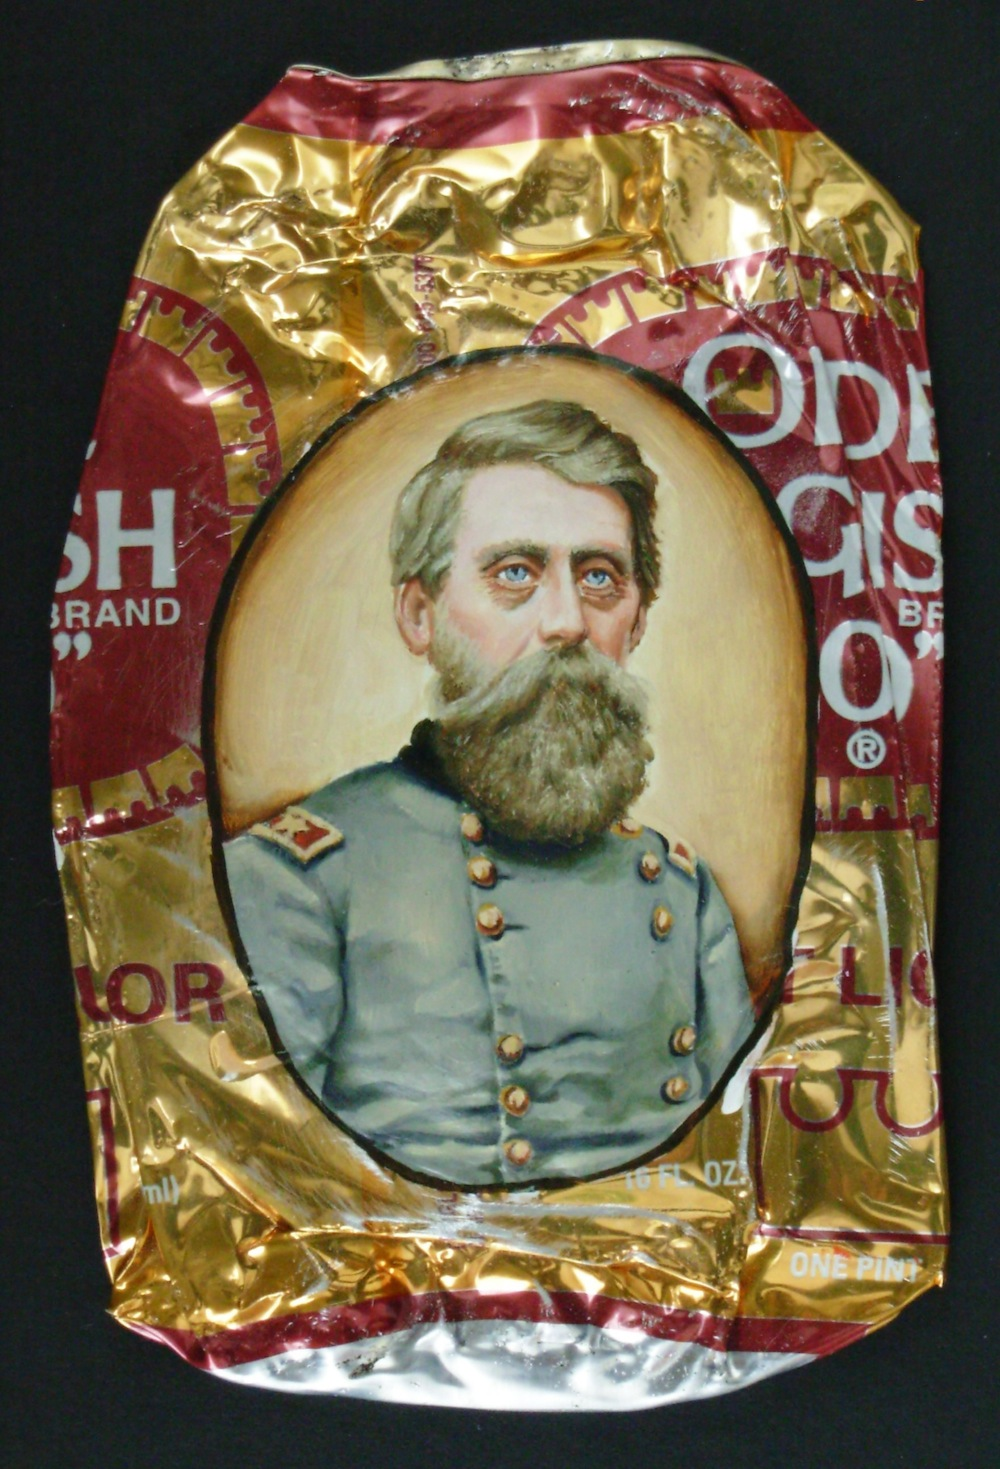
\includegraphics[width=\linewidth]{graphics/Alsbrooks.jpg}
        \caption{The White Trash Series by Kim Alsbrooks}
      \end{wrapfigure}
Kim Alsbrooks, historical oil portraits on flattened beers cans and fast food containers. \quotes{The White Trash Series was developed while living in the South out of frustration with some of the prevailing ideologies, in particular, class distinction. This ideology seems to be based on a combination of myth, biased history and a bizarre sentimentality about old wars and social structures. With the juxtaposition of the portraits from museums, once painted on ivory, now on flattened trash like beer cans and fast food containers, the artist sets out to even the playing field, challenging the perception of the social elite in today’s society.} \quotes{On technique: The trash is found flat, on the street. One cannot flatten the trash. It just doesn't work. It must be found so that there are no wrinkles in the middle and the graphic should be well centered. Then the portraits are found that are complimentary to the particular trash. Generally I depict miniature portraits from the watercolor on ivory era (17th-18th century more or less). The trash is gessoed in the oval shape, image drawn in graphite, painted in oils and varnished.} I need to mention that this images are very subversing to the perception of us about these images. It is unexpected way of presenting images. There is a relationship with the image and painting. At least this work questioned this relation. With tihs work one can ask that with the painting trashed can become valueable thing or with this can this paintiing became valueless. Artsist combines two thing that can be never thought together. New combination, new meaning.}

% Yav biraz da tarihsel fotoğraflara ihtiyaç var mı? aslında bu artworkleri anlatiştaki sıra nasıl olmalı.

% Mandy Barker is an international award winning photographer whose work involving marine plastic debris has received global recognition. The motivation for her work is to raise awareness about plastic pollution in the world's oceans whilst highlighting the harmful affect on marine life and ultimately ourselves.

\item Martin Kaltwasser \& Folke Föbberling: City As a Resource. One Man's Trash Is Another Man's Treasure. Garbage dump or gold mine? The German artistic collaborators Martin Kaltwasser and Folke Köbberling see rubbish as a major resource. Their projects colonize public space in the name of recycling and design: Overnight, they can make pavilions, villages of huts and even whole houses appear. In installations, exhibitions and, most frequently, guerrilla architectural interventions, they question the conditions of urban life as determined by privatization. For example, in a 2004 project called "Hausbau," they built a house in front of West Berlin's infamous Gropius-designed, failed-utopia high-rise development, Gropiustadt, and moved their family into it for a one week stay; for 2005's "Kleinod," they built a bridge and a stairway between a local family's home and a nearby community garden. In City as a Resource: One Man's Trash Is Another Man's Treasure, Köbberling and Kaltwasser propose simple ways of livening up and re-appropriating the urban habitat with sly alternatives to conventional urban planning.

\todo[inline]{One Man's Trash Is Another Man's Treasure. bu kısım rubbish theorydede geçiyordu. bunu bir şekikde sonra kullabilirsin.}

Dump or rich source – the "free materials" discovered on the street, on wasteland and on building site rubbish dumps and recycled by Martin Kaltwasser and Folke Köbberling experience incredible metamorphoses. Pavilions, villages of huts and even whole houses are appearing over night. Since 2002 the artists have been using public space as their field of experiment in projects on the use of (free) resources. In installations, exhibitions and most frequently, in actual interventions they question the conditions of urban life determined by privatisation and economisation. Through realised projects the book reveals simple ways of livening up and re-appropriating the City as a Resource and thus offers new components in an alternative to conventional urban planning. Köbberling and Kaltwasser propose informal and self-organised structures rather than the usual methods emphasising control, security and as much marketing as possible. Their approach demonstrates that often – with the help of their own clever building logistics – a huge impact may be made with a minimum of financing.

% From Hold it! : the art & architecture of public-space-bricolage-resistance-resources-aesthetics of Folke Köbberling and Martin Kaltwasser
Public space is under siege. The compulsion to consume, increased monitoring, and continuous traffic expansion will bring fundamental change to the appearance of cities. In 1998, Folke Kobberling and Martin Kaltwasser began implementing their concept of an artistic and architectural aesthetic of resistance to this appropriation. Using 'structural interventions' in streets, squares, bridges, parks and interior spaces they propose alternatives formed of urban 'waste': litter, trash, and other discarded or donated material. 

Köbberling\&Kaltwasser’s large architectural structures attempt to make visible the value of movement and communication through the transformation of found materials into publicly used objects and spaces. Using the city as a field of artistic experimentation, addressing issues of public space and sustainability, their installations, exhibitions and interventions critically question privatisation and economic pressures. The work will be an act of resistance to occupy and reclaim a space and change its meaning. At the same time, the work mirrors the socio-economic aspect of the city - the city as a resource, the materiality of the city, the free material of a city. 

For their projects they use the “city as a resource” and draw on materials they find in urban spaces, for example in containers or on building sites.

Public space and transformed materials. 

% From: http://www.goethe.de/ins/cz/prj/art/kue/koe/enindex.htm
Public space is under siege: pressure to consume, growing control and more and more traffic are threatening to change the picture of our cities dramatically. The couple Folke Köbberling and Martin Kaltwasser have been elaborating their idea of an artistic and architectonical aesthetics of resistance against this take-over since 1998.

They confront consumerist ideologies with alternatives: structural intervention, artistic statements, actions and theories. In doing so, the artists make use of streets, squares, bridges, parks and interiors as operational spaces. And the material they use is always obtained from urban resources: things that have been thrown away, garbage, donated things.

% Sample phrases
% The topic of recycling, presented in this issue, is the "re-use" of materials, objects and structures, for different purposes, and in different ways from their original uses, in order to build or re-build, to provide possible solutions to problems related to the environment, and to manage waste more intelligently. Tyres, containers, bottles, cans, CD-ROMs and even keyboards, can find new and unexpected uses in experimental architecture, exhibition pavilions, or low-cost housing. With recycled objects, one can build anti-seismic and energy efficient houses. Recycled materials can contribute towards building shelters to meet the needs of people affected by disasters. There are many topics connected to recycling, and they vary depending on the objects that one wishes to recycle and how they will be put to use. Used tyres find many applications in REfunc architecture and the Bohlin-Cywinski-Jackson studio. Dorte Mandrup transformed a piezometer into the supporting structure for apartments built with standardized modules. David Hertz reused the wings of a 747 as roof for a villa in Malibu. TYIN Tegnestue architects restored a building with recycled materials, mainly found on location. Yatin Pandya and Footprints E.A.R.T.H. built an activity centre in Ahmedabad using items that were considered as rubbish to their original owners. James & Mau and Infiniski designed fashion homes with recycled containers. The same kind of containers were used by MacArthur Studio and Means & Wells, to build a travelling exhibition pavilion. The GAD. In London, Folke Koebberling and Martin Kaltwasser constructed an experimental theatre using only recycled materials. The panorama that emerges shows the extreme heterogeneity of the work, materials and techniques, the intuitive approach and the infinite possibilities offered by recycling. All of these projects highlight the importance of the construction process as an opportunity for learning and discussion. 

\end{itemize}


%*****************************************
% Maybe...
% Artistic tactics
% Topology of artworks
%*****************************************


%%%
%%%
%%%
\section{Summary}
Are artworks made from trash just examples of collage and assemblage or more than from them? What about the experience and interaction with other people? Turning art making process to a life practice (or part of life) can be explained in the context of collage (which is mainly related with how a 2d canvas created). But all of them work in fragments, combine many objects together. 

Garbage is often viewed as a form of society’s excess---as the unwanted things that are thrown out without regard. 

In the world of computer science, the term garbage also refers to situations of loss in which data or objects in memory go unused in computer operations.

(Trash has a history. They have different stories. But same destiny?)

Lets make clear the motto: "trash to treasure". What is treasure here. What does it signify? Treasure---something very valuable. from trash. Then it is trash. Not once it is trash. What type of treasure. Who can get value from it. Who creates this treasure? How does it created? Trash is actually is opposite of treasure and then it is switched. In other words trash become treasure and treasure become trash?

Lets consider the practice of working with trash. Why someone believes that discarded objects of people \ldots Looking things that people are refused. Transforming is the one of the most common practice of whole history of man and nature. This practice is forgotten or it is still alive. Agnes Varda actually shows that it is still exist but in different forms. They use it what ruling lifestyle throw out. They are everywhere actually but you should look them carefully. They live in the borders. But live. Event if they are refused they live. Actually it is hard to say that they want to integrate to the system. They want to change it? 

ability of transform, well actually it is very easy to throw away. hard thing is to keep it. force the material. the dimension of trash.

% FROM drink UP, author: Werthan, Sarah, artist: Leech, Gwyneth. A Year in Cups. http://gwynethleech.com/
% trash and art collided. Paper and art, actually paper already medium of art, but is there anything different here. Itself is a part of a work, not the drawing, or painting.
% Documenting via a blog or a website. (what type of dimension it brings the work? maybe connect them, leave message.)
% Buying a beverage is a daily event for \ldots
% Creating art in public places can demystify the process for passers by, Leech says, making artistic expression more accessible and part of people’s everyday lives. The reason of website.
% “People see that an artist can make work anywhere, and make creative spaces anywhere,” she asserts. 

% Trash is as a material or a subject. Both of them. Can be traced examples of artworks.

\begin{itemize}
\item Where do you think this object came from?
\item Why do you think that someone labeled this object as waste?
\item How can you transform this object to tell the story that you thought of before?
\item What story does it tell you?
\item Does it remind you of an event, a specific time in history or in your life, a place, or a state of mind?
\item How can you bring that story to life? (Taylor, 2006, p. 9).
\end{itemize}

% TODO PRAP. from rethink, reimagine, reinvent
\paraphrase{Recycling art approach to using reclaimed objects in artworks requires rethinking, or examining the affordances of a particular object to explore the possibilities for the object's inclusion in an artwork. Assemblage art involves the creation of new and innovative objects from what were once considered objects of waste; that is. through their use in assemblage pieces, reclaimed objects are endowed with a new. sometimes paradoxical meaning. The transformations of the objects used in assemblage pieces ask viewers to reconsider the notion of "valuable" as they are challenged to look at everyday objects with a new perspective (Taylor, 2006). Viewers confront issues relating to the functionality of objects during modern processes of production, consumption and distribution.}

\todo[inline]{Artifact exploration promotes historical thinking, literacy investigation, and cultural expression (Higgs \& McNeal, 2006; Levstik \& Barton, 2001; Morris, 1998). Meanings are embedded within cultural artifacts and language (Vygotsky, 1978).}

%%
%%
\subsection{What might be the meaning of using trash as a medium in the artworks? Questioning trash as a medium for artist}
\begin{itemize}
\item Some works try to raise awareness the problems that are the result of trash. (It treats environment and nature.)
\item Some of them reflect people's lifestyle especially throw away culture. As a mirror of current lifestyle.
\item Try to find a new value and meaning from the discarded material that are useless anymore. To explore a new approach, new way. Subvert people's ideas about trash and their attitudes by turning materials to the something meaningful (or valuable). Trash to treasure.
\item Using discarded item to represent other discarded things by the ruling ideology or approach. For example, trash can be used to represent refugees. The things that we are trying to discard does not mean that they have no value, instead it means that we have no ability to reveal its potential. In other words, refugees have potential but we see them as players that will change our current system. Therefore, it can be said that willing to transform trash to treasure is to require change of current lifestyle. Rejecting discarding something especially thing that you get value from it is a process and spread through to the ones life.
\item One way is not to produce trash. (Zero trash philosophy.) The other one is to transform trash into something else.
\item What type of experience is that collecting and working on objects that are generally discarded? Experiencing out of common practice, being open to new explorations.
\item Instead of a world that produce trash, how could it be a world created from trash?
\item Combining industrial goods with objects transformed from trash is another way to find a place to trash in the community. It also signifies that trash still has a good quality to used with new materials. Creating composite products from new and reused items. Using the valuable thing with the invaluable thing. It becomes more valuable or less valuable. Depends on the perception.
\item Aesthetics of trash. Revealing aesthetics value of discarded stuff. (Unique visual value. Trash portraits, sculptures etc.)
\end{itemize}

Artists works and the place of the trash in the art can be summarized as follow:
\begin{itemize}
\item Artist see them as potential. But what type potential it haves. In which areas. They are already thrown away, if it was value or has a place in the current system they are not thrown away. There is an alternative life and outside of the ruling system.
\item Visual uniqueness, aesthetics dimension.
\end{itemize}

% Ben bölümde aslında çöpün sanatta nasıl yer aldığına bakıyor olacağım. İlk kim kullanmış nasıl kullanmış. Sonrasında hangi anlamlarda kullanılmış. 

% Aslında ben uygun her yerde çöpe olan yaklaşımlarla ilgili örnekler verdim. Peki ya bu bölümde ne yapacağım. Belki gene değineceğim. Ya da ne anlamlara geldiklerini özetleyeceğim. 

% Hangi sonuçlar çıkacak aslında bu bölümden benim için kıymetli olan o. Özellikle caselerden. Bu nasıl bir artistict act oluyor.

% Her sanatçı bu arada çöpü dönüştürmüyor. Bazıları ise onu oldukları gibi kullanıyorlar. Yani farklı kullanım seneryoları var. Ama ben dönüştürmeye dair ne çıkaracağım bu bölümde. 

% aslında dönüştüğünü nereden iddia edebilirim. Rubbish theory? Durable state. Ya da onun tekrar hayata geçtiği. Benimkiler de belli noktalarda fösterilecekler. İnsanlar o defterleri saklıyorlar ne de olsa. Zaten dönüşme işlemi direk müzeye çıkmasıyla oluyor. İllaha onun materyal olarak dönüşmesi gerekmiyor. Bu yüzden her iş aslında bir şekilde dönüştürüyor. Sanatsal pratikler çöpü dönüştürüyorlar. 

% Sanatsal bir eylem olduğuna nasıl varacağım peki? Çünkü topluyorsun, belli bir yaklaşım geliştiriyorsun. Bu eyleme insanları davet ediyorsun. Sanatın eylem olma olayı... Buna burda değinip, kendi işime geçmeliyim.

% Ne topladım buradan. Bu işin sanatsal bağlamdaki yerini öğrendik, yaklaşımları öğrendik. Yeni ihtimaller görme, hayatta var olma, alternatif oluşturma gibi. Ben de bu tür şeyleri kendi işimde kullanacağım.

Childs can enjoy with trash. I remember from my childhood, we collect crown cap and play with them. Some caps are found less and they worth more. We are looking everywhere for them. To make them flat we put them on the railways. After train passed we get perfect plat cap. At that time it is not trash for us. It has a value and part of our games and enjoy. To have fun a bunch of trash can be enough for us.

Think a city that has trash monument in the every corner. created from their trash. merged with the city life and gaining unique cityscapes and aesthetics. or think that a museum a trash museum. Exhibits works of art embracing the trash in all aspects. Maybe done by the artist or the visitors from all around world. A place for garbage other than a landfill. Waiting their creator to meet again. What a great idea isn't it? Meeting their creators again. But this time their creator can recognize their trash. They transformed to totally new thing. Reborn. Transformed (Kafka, Gregor Samsa).

\todo[inline]{Overview of all artworks. How do they differ from each other in terms of transformation(conceptually, physically), methodology, collecting, composition and so on.}

\todo{a chart here.}

\textbf{Resim tahtası.} Bazı işler çöpleri kendi işleri için bir kanvasa dönüştürmüşler. Çay poşetlerini boyayan kadın, Kitapları boyayanlar, teneke kutuları boyayanlar. Hepsi aslında kullandığı ürünle farklı bir ilişki kuruyor. Onları farklı bir hale getiriyor.  

toplumun davranışlarına karşı bir cevap, görülmeyen, veya farkedilemeyen unutulup giden bir hale getiriyor.


\chapter{Thesis Project: Notebooks from Trashed Papers}


%****************************************
% Structure of Chapter:
% 
% Artist Statement
% Development of Work
%  Collecting, Transforming, Tests...
%
% Final Work
%  - Notebooks
%  - Website
%  - Exhibition
%........................................


%****************************************
% Relationship between my project and theoretical aspects:
% - First one is actually is to analyze what is trash? Because I am using trash material and what is point of view of scholars to the trash. Realizing the potentials of it. Also the difference comes from the working on virgin object and trash object. Understanding the difference between the bricolouer and engineer. If trash has multiple life than these research will somehow reveal it. It is actually research on trash but what purposes. I guess it is missing? I need to set a purpose for the theory chapter. Or it is a just a background chapter? 
% - Roots in the art history. (Also roots on the social life can be researched?)
% - Inspiration from the other artist and also 
%........................................


%****************************************
% Sample Phrases
% \ldots is the concern of this study which aims to \ldots
% The aim is not to practice Antiquarian Avant-Garde techniques as a puritan form of photography, but rather to envision new means of photography.
% The aim of the thesis paper is to historically, socially and theoretically contextualize a student's work. The written thesis documents and informs the development and resolution of each student's artistic practice during the MFA program.
%........................................


% FROM Wild Art. quote taken from the television series `American Masters', Season 5, Episode 8, John Cage: I have nothing to say and I am saying it (aired on 17 September 1990).
\epigraph{The first question I ask myself when something doesn't seem to be beautiful is why do I think it's not beautiful? And very shortly you discover that there is no reason. If we can conquer that dislike, or begin to like what we did dislike, then the world is more open. That path ---of increasing one's enjoyment of life--- is the path, I think, we all best take: to use art not as self-expression, but as self-alteration; to become more open.}{\hfill---John Cage, \textit{Wild Art}}


In this chapter the artwork(thesis project) will be explained in detail. Final work and it's progress will be explained. Connection will be established with the previous chapters. Stages of work and concerns will be explained. 

% What I have write is here to cover the project can not be sufficient. Because it is not possible to say everything about this project. I wish that this work would allow different interpretation and readings. 


% TODO
% Felix Gonzales Torres'in untitled işi benim yapmaya çalıştığım ile ilgili.


%%%
%%%
%%% 
% TODO
\section{Artist Statement}
(Collect, Save, Transform, Spread.)(Rescue, Revive)

% Closest waste bin is actually my own pocket.

% Converting disposal things to multiple time usage. Realizing the alternative lives of trash beyond their defined one shot life. Giving attention to the things. 

% Eğer bir artistic actten bahsediyorsak sadece bunun ürünle değil, üretimi ve insanların dahil olmasıyla desteklenebilir. Zaten toplama sürecinde bunu insanlarla ilişki kurarak yapıyorum. O insanlarda diğerleriyle konuşarak yapıyorlar.

% At this stage it is claimed that the process of transformation of trash can be treated as artistic act. In the production of notebooks people collected papers from different places and location. During the collection phase they also collect them from other people. In other words there is human communication during this process.

Actually (It is questioned that) working with trash dictates a life practice and, it is a convergence of behavioral patterns (attitudes toward to trash) and art making. The process effects one's life and lifestyle. (But what type of interaction between life and art making process?) (This claim is the main driving force of my artwork which is part of a thesis.) The purpose is not to build a thing that is produced from discarded material to watch it from a distance. The important thing is to interact with it. Because it is already discarded (disgusting, abject, unattractive etc.) and general behavior avoid from it, this work must change it. It must call the viewer to interact with it.

% Ersan hoca uzak seyretmek yerine etkileşime geçilmesini auranın kırılması olarak bakıyor. Performatif olması veya bir act olması zaten bunu kıran bir şey olabilir. Sanatsal eylem, performans kavramlarını araştırmak gerekli. Uzaktan seyredip hayranlık duymak yerine ilişkiye geçilen bir hale getirmek çöpü. Amaç bu aslında. Çöpü tekrar tanımak, onunla barışmak, onunla yaşamak. İşte bu yüzden bir eylem olabilir. Ya da yaşam pratiği. 

% Olay sadece böyle çöpten bir şeyler yapıp insanların seyretmesi değil, mühim olan onunla iletişime, ilişkeye geçmek. Yani zaten uzak durulan bir şey, onlardan bir şey üretildiğinde izleyici gene uzağında duruyorsa ne anlamı kaldı ki? İnsanların bu işin aşamalarının bir parçası olmalılar.

With the help of art (and artistic practices) discarded things can find a place in the society. (By the help of artistic approach things can be gain new values and meaning even if they are discarded and excluded from daily life (or society). The relationship between value creation and artistic practice examined through the artworks that uses trash as medium.)

% Using trash can not only understand in ecological perceptions, it also have powerful political claims. Or it should be examined in deeper levels beyond collage and assemblage, the medium itself has different meanings. 

% SEEING IT AS A RESOURCE.
Junk(or trash) can be seen as a new resource that is fertile to new meanings, creations and aesthetics. Ignored and discarded nature of garbage when rethought becomes fertile resource. Trash as a resource (as an artistic material). (City as a resource. Seeing the discarded items as a resource. Many artist approach to trash as resource. It is a shared approach. Some of them collect city discard, some of them tea cups, tea bags, discarded papers.)

% Çöpü tekrar ele alıp bir şeyler üretmek, onu tekrar yaşamımıza sokmak yeni alternatifler sunacaktır.

Do she/he want to take back (or revisit) the trash once thrown away? People do not want to think of what they throw away. Turning them to a things that worth to look again. How do artists reflect garbage and what are their tactics? What is the thing that add value to trash and what is the role of art in that?

With the help of art discarded things ---in the scope of thesis in particular paper trash--- can be transformed beyond the other industrial (or technological) methods. In other words autistics practices generates applies different methods.


%%%
%%%
%%%
%\section{Inspired Works}
%There are some works that inspire me a lot when developing the work. They are not actually trash related works therefore I put them in different section and here before the details of my work. However the previous chapter has also very inspirational contributions to the my work. They helped the understand the topic and develop an approach to the topic. In this section some projects are mentioned and their methodologies are explained. How are these works effected my work. What is the relationship between them? (Maybe all of them can be explained only the related part of it.)
%SketchBook Project. Inspires me a lot. Lots of works from all over the world. Full of creativity and showcase of richness of people's expressions on the small notebooks. My work can be considered as a sketch book project through trash. Sketches or only creative progress is not the only consideration. You can send your lecture notes. 


%%%
%%%
%%%
\section{Development of Work}
Here stages(progress) of my artwork are listed:

\begin{itemize}
\item \textbf{Memories.} As far as I know I collect things it is hard to say collecting started after an exact event or time but there are several memories that I remember. One of these (First of them) is from my primary school teacher. When I was third class my teacher give us a homework to bring colorful paper to make something(whatever it is I don't remember). The day after we bring some colorful paper but she did not. Instead of this she bring paper cut out from packages that are colorful, shinny and qualify. And I remember clearly that she suggest that same for us. Do not throw out packages, look for the useful parts and keep them to use later. 
\item \textbf{Motivation.} I can not throw them away. When I throw them I became sad for them. I have to find something useful for it. Even if I can not find it, I can pass it to another person who can make use of it for own purposes. We are humans that can produce, transform items. One of most developed species in the earth that produce and use tools. There is a lot of effort to produce thrown away and it seems that all this efforts are wasted. What I mention is not related about ultimate productivity. It is more close to being thoughtful, and taking responsibility of tools, items and objects that we are using. Rather than throwing out, creating a way that all are have chance to live together is much more close to my perception. 
\item \textbf{Collecting.} One of the most found trash in my habitat is paper. I work at METU Technopolis, live at 100. yil which is the nearest settlement to METU and study at Bilkent. People live there commonly use paper and needs paper. Paper is nearly everywhere. Reusing the paper is not limited with recycling of it. There is a another ways of it. When we recycle them actually we again send away them and use it as we all know. (industrial papers and notebooks.) There is no richness here. Same type of paper. Produced after a industrial process. I collected them from my friends (people that have communicate often). Sometimes I collect them from trash bins and roads. 

\comment{COLLECTING TRASH.} One of the most important parts of the using trash in the artwork (or expressing something, or representation) is to collect them. What are the dynamics(considerations) of collecting them? (easily accessible materials or unique items.) Where to store them? Does it mean that live with trash? In other words collecting trash and using them is live with them? (making them part of life.) After the being part of the are they still trash? Can be thought that it is something that affects the lifestyle. (possessions and trash.) Another question is that how differs collecting trash from collecting other things such as objects that have archival value. What is the driving force? You may collect it to prevent object being lost. For archival things what you collect is something that has some sort of social use and meaning which is going to disappear. However, trash is never disappearing, even its amount increasing rapidly. For archival things people have memories with them, but does some applies for the trash? Who wants to keep trash? or who wants to re-see(re-visit) trash again (in a museum for example)?

\todo[inline]{What type of collecting? How differs from the others? ragpickers from benjamin and archades project.}

\todo[inline]{yaptığım işten diğerlerine referans vermek gerekli.}

\item \textbf{Transforming.} I turned them to notebooks. Actually I use it for my self. And while I was using of it I am very proud of it. I am studying nearly more 20 twenty years and I have always need for notebooks and use them. It is some sort of passion for me notebooks. Because I always admire notebook beautifully design or uniquely designed. I collect them whenever I find and most of the time I only save them for later use. 
\end{itemize}

\subsection{Collecting}

[Organazing People] Well I  actually follow very simple methods. I just talk them all. I explain what I did, ask for their help. Everyone actually approached positively and somehow they contributed the project.

\subsubsection{Collected Materials}
There are different papers and objects are used to produce papers
\begin{itemize}
\item Burger King packages, from office at launch time
\item Starbucks packages, from supervisor, office and my friend. Especially my supervisor and friend collect them from their friends and their own uses. They save them for me and later I take them later. 
\item Modshifters papers, that are covered on table and at the end of the day they are cut out and throw away. I go this place many times and every time questioned what they are doing to the papers. One of my visit we stay there at a late time and catch the garson collecting the old papers and prepearing tables to the next customer or day. I ask him to give me and he kindly accepted. From this paper I covered [x] notebooks. All of them contains track of people who sit down there. I do not know them and I am not sure that the paper that they are sit down turned to such a thing. 
\item Varuna Gezgin
\item Graduation banner
\item Tea bags.
\item Banka sıra fişleri.
\item Elginden gelen kağıtlar.
\item Bilent kağıtları?
% It is also realization of materials. Establishing different connection to them. Why is important? Identity construction.
\end{itemize}

\subsection{Experiments}
\todo[inline]{experiments with paper.}

[EXHIBITION] Starting point is to stack the notebooks onto the each other, and there are some ideas like putting them inside a waste bin to re-do the action of throwing away. Again the purpose is to find a way that to shock people, surprise them. After ward somehow they should understand that these notebooks can be taken. \comment{I set up makets and try some installations of it. Take photo it. listed them here.}

\todo{images are here.}

I imagine a exhibition environment and place notebooks \comment{üst üste.} Different placement are tried. All of them are look like sculptural. I have insert no special meaning as sculpture to this object an I also I am afraid that people does not close them to the notebooks and look them away. which I do not want. 

\todo[inline]{bir de aynı zamanda işin süreci, defterlerin yapımları hakkında bilgi vermem gerekli.}

%%
%%
\subsection{Problems}
There are a lot of questions and problems that I have to overcome while development of my work. 

% Yani aslında bir derdim ve yapmak istediğim bir şey var. Ama bunu gerçekleştirmek için yapmam gereken şeyler var. Ve bunların bazılarının nasıl yapılacağı çok belli değil. Ben bunlara bir çözüm buluyorum. Bir yöntem üretiyorum. Bu kısımda aslında bunlardan bahsediyorum.

\begin{itemize}
\item First one is that my art work can be considered as design and has functional purposes. (It is not just a design, it is uses design to reach its goal like many artworks use other disciplines to reach their goals and expression. Purpose is not design and functionality.)
\item Using unused industrial paper. (Mixed trash and virgin material, \textbf{to show that discarded and desired object can live together.})
\item Collecting them with help of people, and asking other people to give the unused papers. (Collected from my close friends, from supervisor, from office where I work, from modshifters and varuna gezgin and from bcc labs(hopefully)?)
\item Giving them to people, but people should take them voluntarily.
\end{itemize}

\subsubsection{Functionality and Art Debate}
From an art historical perspective, you could say that functional art is the inverse of Marcel Duchamp's famous readymades, where he transformed utilitarian objects---a urinal, a bottle rack, etc.---into conceptual artworks by fiat: it became art because he said it was. Duchamp's works kills the functionality. It works beyond the functional perception. Moves the debate to the conceptual frame. However it is not every time case. Today many functional art objects are as avidly acquired by collectors as their fine-art brethren, and are appreciated just as much for their beauty as their use value. Ancient Chinese vases, for example, while still capable of performing their originally intended function (displaying flowers), are prized for their historic and aesthetic value more than anything else. \quotes{In conceptual art,} Sol LeWitt writes, \quotes{the idea or concept is the most important aspect of the work\ldots The idea becomes the machine that makes the art} \cite{lewitt1967paragraphs}. Therefore anything can be turned to art with a good idea. 

\comment{Comparing art to craft is like comparing philosophy to engineering: they're two separate ways of looking at the same thing. To me art is communication of an idea or an emotion, while craft is the physical manipulation of material. An object can easily be both, either, or neither. A sculpture, for example, may communicate, but it was constructed using craft. Likewise a teapot can communicate an idea, but it was crafted. Function is misleading and no distinction. Functional objects can still communicate ideas, so art can be functional. One object could be viewed two ways: if you look at the way it was made and the materials used, you are looking at its craft, if you think about its ideas, you are viewing it as art. An object could have been crafted, but contain no art. Even a painting can be crafted but artless. A ready-made might be art with no craft. I very much like the idea of a spectrum. One last thought: skill doesn't enter into the definition of art, since a piece could succeed as art but be poorly crafted.}

\textbf{Why is it not a design?} Because the considerations and priorities are different? Functionality is not my primary concern. I do not increase the functionality or searching best functionality? (Considerations of design and art can be compared and what are my priorities in this work. I'm not trying to finish the garbage problem. Is it a problem for me? Do I problematize it?) 

\textbf{Why is it art?} Uses artistic methods? Does it represent anything? The idea is transforming things. Anything can be transformed and re-contextualized again. The limitation is our imagination and approach. It has a claim. In can be analyzed and examined in the context of art. It is hard to say that something is art or not. However it can be examined in the context of art. There are artworks reject art galleries. There are artworks also reject commodities. It has purpose that. spread out the idea in different manner. Subverts peoples ideas. 

The work aims to liberate the imagination and change the way people see the trash.

%%
%%
\subsection{Paper}
"Paper is an indispensable product throughout the world. Its primary use is as a medium for writing, essential for bureaucracy, education, communications, information storage, and in the spread of information. In addition, it is used for the packaging for transport and convenience of a wide range of items from food to industrial equipment. Paper also has specific technological uses, such as for filters and in art, home furnishings, and architecture, and it has a range of uses for hygiene purposes. Paper in several forms is consumed on a daily basis by each person in the Western world." \cite{trafford2012paper}

\comment{My experience here: For example when i collect the papers under the dishes or food packages, people often thinks that it is disgusting and call them as dirty. But it is very strange that the fat on the paper is previously what they are eat.}

Paper is both biodegradable and a renewable resource, which means in consumption and waste terms, its environmental impact is relatively small compared to the many more-toxic and bulky waste products that are found in everyday garbage. However, the chemicals, water, and electricity used in its manufacture are considerable---and these are nonrenewable resources---and certain types of chemicals used in paper production are toxic. In addition, if waste paper is sent to a landfill, it releases carbon dioxide emissions. Further, forest resources are not always as renewable as one may like to think. These environmental impacts can be greatly reduced by recycling (paper being one of the most easily and cheaply recyclable products in everyday use) and by conscientious consumption practices.

Paper made exclusively from wood is called virgin paper, while paper produced out of used paper that is re-pulped is called recycled paper. Recycling paper can greatly diminish demand for virgin fiber from wood. However, there will always be a demand for virgin paper because, although paper is thought of as a renewable resource, it cannot be recycled indefinitely. It can only be recycled four to six times, as the fibers get shorter and weaker each time. In addition, some virgin pulp must be introduced into the process each time to maintain the strength and quality of the fiber, so no matter how much is recycled, paper will always need some virgin fiber.

% History of Paper
The word paper comes from papyrus, the plant that was first used for making a medium for writing in ancient Egypt.

% Production of Paper
All types and qualities of paper share the same basic method of manufacture, including newspaper paper, print paper, and carton used for boxes.

% Uses of Paper
Paper has become the most ubiquitous product in the age of information. Such products often complete their journey from shop floor to garbage in a single day; for example, newspapers, print paper, packaging, lavatory paper, tea bags, transport tickets, price tags, shopping bags, flyers, leaflets, wrapping paper, napkins, and tissues. 

%%
%%
\subsection{Why (package) paper?}
Easy to collect. Easy to find. Thrown out even if it is good quality. Packaging materials are very widespread. Appropriate for painting and writing. Has a very short life time. Disposable, there are a lot of package outside. No need to carry it. Every place gives you package paper. 

%%
%%
\subsection{Why covering notebooks and books?}
They are all package paper, already used as carry things and this work it has used again for the same purpose (but in different connection, this time trash is bound to the notebook). Trash is used to cover the papers. Cover is the most visible part of the notebook and book. Therefore trash becomes most visible part of the produced item. What is the function of cover? It gives ideas about what is inside, distinguishes from other things, protect it.

%%
%%
\subsection{Why giving away?}
Aim is to spread the idea by making something useful from trash. Increase diversity, activate (or encourage) people to embrace the trash.

%%
%%
\subsection{Why in the public space?}
To reach more audience. Actually the audience is out of the art galleries. They are walking in the streets. Putting them to next to people is much more effective. It is not visible and nearly it is hided from society. It is dirty. Removed from the society. There is a effort to hide them away. However in this project it is again showed to the society. Because it is revisited and reclaimed. 


%%
%%
\subsection{Artistic tactics}
Here I followed some tactics to realize my purposes. I called them artistic tactics. Easy to carry while traveling. Small notebooks. Placing them to their routes. 

\subsection{How I reached to notebook?}
Actually I have been collecting same materials that are used in my project before the thesis work. In my mind there is always belief that I can I find something useful for them. (In that time my main evaluation was to create useful object for my need.) Later it turned to an artwork. Before the thesis I also produce the notebooks for myself. However what is changed in thesis. First my approach to the trash is a little bit deeper. What is added to the notebooks. I started to use also used papers. for the cover of the notebook, I use more different materials. more close to collage. production method changed. and I started to collect different things, from different places. My realization increased. I organized my close friends and others to collect or save their trash for me. I discovered some points. their differences. 

% What I tried during this progress: Wrap out the trees, because I think that most of the materials that I collected are package papers. Well I somehow package the trees again. not to carry them but to raise awareness. Yani benim amacımı en iyi anlatacak olan şey nedir? Aslında ben burada defterden gidip bunu anlamlandırmaya çalıştım. Dolayısıyla deneyerek deftere nasıl ulaştım da ziyade defterden başlayıp nasıl tekrar defterde karar kıldığımı anlatan bir hikaye olabilir? Yani bu çok da şart olmayabilir bir diğer yandan da? Developlement of work? Nasıldı nereye geldi? How my project evolved? And this also explains how it is relates with the research. Because the reasearch is shaped the project also. Which part of the project shaped by the project? Not thinking in the ecological perspective. Raised questions also mature the project? For example zizek suggest that to find spirutuality and aesthetics to the trash, and for me? 

\textbf{Why notebook?} Because I already do it. So What I didn't change it. It is the best one or no to change it. I love idea of carrying notebook with near of you. I have also save my notebooks. I don't throw away them. A notebook is actually is a work of you. It carries your signature. It is one of best gift to give someone. Because it is a combination of your work and the other peoples works. It is co-authored work. Actually there is also a part of people who throw away this peace. Actually the best part of it the transformation is not finishes after my creation of notebook. It continues with the usage of it. How it turned to is not actually uncertain. Therefore it is very appropriate of my idea that transforming trash is increases the diversity.

\textbf{What is different from industrial notebooks?} Handmade, from trash. an alternative to other versions. every one have different stories, they are different in visuals (but the others are also different.) What makes them different is not clear actually. Does it have to be different? Yes. The production method is different. You pay no money. There is different with gift notebooks from companies. This notebooks call to you change the destiny of trash together. 

\subsection{What do I think about trash?}
I need to clarify my approach to the trash, wasting and discarding. First point is that I am very uncomfortable to the action of discarding thing. I always think that by discarding this think I am missing something rather than getting rid of something. Sometimes because of the significant amount of residue from consumption from daily activities I became overwhelmed and to move on I need to leave behind them and move on. However almost it is never ending loop. (I believe that sometimes we need to break the loops to realize different meanings. To think outside the box, we need to behave outside of common habits. As I mentioned the discarding things are some of the loops that we are rare to behave like other way.) \textbf{What am I discarding?} To get rid of my load and move on. But for what? and also ought to be like that? (throw away them to same bin. (Some of people do not care too much bin and throw them whenever it is possible.)) Even if I discard some stuff I think that I am ignoring its potential and losing it. At that times I become very sad and feel very comfortable. I must have find to another place for it more suitable than a waste bin. At least I can give them someone else who can use it for own purposes. Do I really luxury of discard?

Significance of thinking outside the box (about actually trash) is actually breaking the loops. You have to look at differently from your common perception. \textbf{Break the rules, break the loops.}

\textbf{Making exploration.} One of the encouraging factor is to work on trash is to find (or explore) something different from someone else's discard. Because it is discarded and undiscovered. Wait us to be discarded. and possible (as picasso mentioned) discovered again and again. 

\section{Parts of project (or final work)}
The project introduced in this thesis have different parts. Each of them are connected to have relation with and support the other. Different parts also enable us that different level of integration to the project. 

\subsection{Notebooks}
Mixing materials is main method in the production process. I combine different papers and packages. I try to generate every possible combination. For some of them I establish the connection but for the others the connection is not obvious but it is not obligatory. Because trash is state where you can find meaning through the trash or material later. 

All package papers are cleaned up. Because it is important that it needs to be safe to use. With mix of water and little bleach they are swabbed. 

\subsubsection{Name of notebooks}
  \begin{figure}[ht]
      \centering
      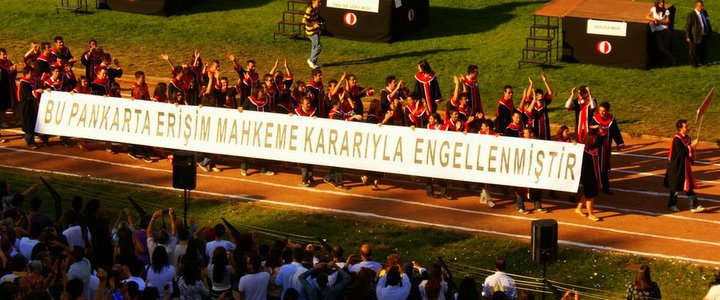
\includegraphics[width=0.8\textwidth]{project_graphics/banner1.jpg}
      \caption{Banner}
      \label{fig:Banner_1}
  \end{figure}
\begin{itemize}
\item \textbf{Puzzle.} Because it is cut out from very big and long banner (which is carried at graduation ceremony at METU, 2011). Every piece was a part of bigger banner. At that time there are serious debates about freedom on the internet. Most of the website are banned from the decision to the courts and they were not accessible. (Access to this banner is blocked by a court decision.) In Middle East Technical University there is a tradition that in graduation ceremony people walk through in the stadium and greet to the tribunes. With this event they carry some banners to express their feelings and criticize some realities in the country. This one of them. It is carried by students (new grads of Computer Engineering) The slogan decided by among the students and before the ceremony I printed out the slogan to carried out as many people as it can and easy to readable from the people who seat at the tribunes. After the ceremony I could not throw away this banner. I do not know what to do it, it is very big actually to store but I could not. I think that I will figure out later. Maybe I can use it as a draft paper. But is it worth to cut out this all long banner etc. Also to strengthen the banner and to prevent to tear while carried by the many people we are tape it from its boundaries. In other words some of the areas can not appropriate for writing. When I decided to this topic I remembered to this banner. It is stands in a corner in a dusty way. Now it is time use it. It waited very log time and it is time to revive again. Currently In turkey the problem of banning web-sites continues. Event it can said that people do not surprises when a website is blocked by the courts. It can be turn be a paper that people can freely express their ideas and feeling onto the it. Cut out them to the smaller pieces and make them as notebooks. They are part of puzzle. for the smaller parts what is written on them can not easily understandable. To realize what is the message is you have to bring together all of them again. But It is not possible, therefore website is a very good solution for them. All pages have unique patterns. Remaining parts of letter and tape. It provides unique layout for writing and I strongly think that all the notebooks after used have strong visual impact. 
\item \textbf{12:00 pm.} Burger King pockets from office where I work. Because it is launch time. It is collected at the same time.
\item \textbf{08:00 am.} Breakfast time. I think that these packages are used at the morning, very the beginning of the day.
\item \textbf{Friday Night.} (Maybe there can be another option related with traveling, or union). These notebook's pages are collected from restaurant "Varuna Gezgin". We go there to meet some friends after long time. One of them is coming from Australia, the other one is coming from Norway. they are my friends from the university. We united again at varuna gezgin. The place also interesting story. It is a place of travelers. It supports them. and the decoration of that place contains a lot of items collected from different sides of the world. The concept of the place and our meeting perfectly matched. I'm collecting the paper that are under the plates. When we are leaving this place, I ask the guy at the desk, I am making small notebooks and is it possible to exhibit there. I said that is it possible to give them to people. Firstly he asked me that selling them but I said no they are free and part of my thesis project. and later he offered me there are a lot of unused papers. I can give you. they are not used and waiting to be recycling. I took some of the papers, and that papers are part the sheets of these papers. 
% Name of the paper can be related with this place and related with the meaning. 
% Again I need some memory from here. 
% They are all my memories actually and I also turn my memories something different. Changing and constructing memories. And also others' memories... These project also contains others memories.

% Ersan hoca's packages. Elgins' papers etc. I do not know actually their stories. Maybe I can dream up stories for them. Creating histories from some of the trashes. They do not have proper memory with me, but I tried to construct memories, (fake memories can be said that.)

% Refer to 9 canlı. Never dies, revives again and again. Because trash moves in the community, even if thrown away can be find another use.

\end{itemize}

\subsection{Exhibition spaces}
Especially it is the most hard topic in the development of the thesis. To find a place for the notebooks is great issue for me? 

\begin{itemize}
\item Library. The reason why select library is there are small papers to write down the location of books. Libraries are places that things are reused. Books are used by many people. It is place of sharing culture. Books are shared by all the other peoples. 
\todo[inline]{problematic because of resusing. actually is sharing.}
Bilkent, METU, Milli Kütüphane. Buraya nasıl gidilecek. Ama öncelik zaten bilkent kütüphanesinde. ODTÜ sonra geliyor. 
\item Torun. as an alternative place?
\end{itemize}

\subsection{Website}
As I think that finding a place the discarded items is one of the main purposes of this project. As it finds a place peoples life again, it also finds another place in the digital space. ()

Mainly websites displays the story(History) of notebooks. Also it is a place to track the journey the notebooks. As I claimed that it is not a finished work. It does not completed transformation. It always continues. Therefore a website that anyone can reach share their progress via website. Anyone can later discover how they turned to new things etc. 

Collect peoples comment with this notebooks. As I leave notebooks different places I do not have connection with people who take them. This website also will help to collect/share peoples ideas about the notebooks.

It will contains a section for how notebooks are produced and the story behind it. The purpose is to record the creative process and share with the others. Revealing the process is significant to demystifiying the truth about the project. It makes it more clear that the object used here is actually transformed from something else. 

\textbf{Why website?} Maybe you can think that there are different methods to accomplish recording and sharing the process. In a gallery on a single table or a room it can be succeed. However it like the idea that website can evolve by time as this work evolve in time. I think it matches perfectly. This is not a finished work, it continues and so the website also. 

% Meaning of stories behind the process
There are different stories behind the objects. I try to record their stories (by photography and taking notes) but some of them were not possible. However I still use them in the work because even if I missed their story, with their materiality reveals their history. It still has a history but needs to rewritten. Maybe forgetting all the history maybe creates different notebook.

It is also co-authored work. Because many people helped me to collect the papers and also many people leave their trail to the paper and also they bring meaning to the them. After production of papers I also want them to continue as co-authored process. In other words many people will be part of this project. As people see different things on objects and bring them to me. the variety of things is increased in time. Because people sad me that \quotes{I thought that you can use it. Do you collect also these?}. After that time I want to continue as so. 

% I add the screenshoots of website. Also the development of it. Sketches of website. Navigation of it. User interaction. Use cases and actions. Functionalities.

% Documenting the progress. 

% It was not only that such characteristic was clearly suited for the exploration of human spaces such as home, but it was also that I am comfortably and confidently fluent in practicing photography

% Counter Argument:
% People may think and raise the question that none of notebooks is actually my work they belongs to others, others(Starbucks, Burger King) designed it and I am stealing their work. Here there are available different answers to the question. Firstly they are different once they are designed. Turned to different thing. I suggest that them to consider in different context like Duchamp. 

% I resurrect things that have been killed off... My work is all about the potential of materials — even when it looks like they've lost all possibilities. (Cornelia Parker) https://en.wikipedia.org/wiki/Cornelia_Parker

% These all memories and collected materials related with the my history. So why is it important for the other people. What can they found my memories. This is not theirs. How other people connect to the topic. They important for me but also I need to find something important for the other people. For example modshifter and varuna gezgin is one of them. This not only my experience. Some kind of shared memories and histories. What will find people in these notebooks.


%****************************************
% EXHIBITION
% Where people access them? How to design the experience here. The relationship with the location? 
% Pizza box, with l shape box. I need to find a place to put them. 
%
%........................................


%****************************************
%% Move to the other sections:
%
% Mandy Barker is an international award winning photographer whose work involving marine plastic debris has received global recognition. The motivation for her work is to raise awareness about plastic pollution in the world's oceans whilst highlighting the harmful affect on marine life and ultimately ourselves.
%........................................


%****************************************
% TODO Find a solution for this problem:
% Bu işin olması için ben insanlardan bir şeyler yapmalarını istiyorum. Yani aslında kendimde yapabilirim ama neden insanları da dahil ediyorum? Buradaki en önemli amaç değiştirmek dönüştürmek, sadece çöpü dönüştürmek yetmez, insanların fikirlerini de deönüştürmek gerekmek. ve bu bir süreç işi (şart mı tek bir yöntem bu mu?) İnsanlar nasıl değişir diye sormak gerekir o zaman. İnsanların değiştiğini dönüştüğünü gerçekten nasıl ölçeceğim ki? 

% important question: herkes neye ihtiyacı var ise onu toplar. ben neden niçin topluyorum. toplama sebepleri. dönüştürme sebepleri. neden sadece toplamakla yetinmiyorum. yani toplamak ile ayrıldığı noktalar nelerdir. Ben bir mana mı arıyorum? Yoksa kaybetmekten mi korkuyorum? Yeni kompozisyonlar oluşturmak istiyorum. Farklı karşımlar elde etmek istiyorum. Bir tür şaşırtmak durumu... Beklenmeyeni yapmak... En olmadık malzeme çöple çalışmak bu yüzden önemli benim için. 

%
% PROBLEM:
% In theoratical part I am focusing on actually the trash. But should I focus on paper trash? Is there any difference? Ya da ben oradaki bir farklılıktan besleniyor muyum? It is not totally paper, actually they are package. Examples can be given related with package material. It has a very short life. Not short actually. 

% How to establish the relationship between the collaboration and the trash? transforming them with the help of people. However, main discussion is not about collaboration. Here collaboration is a method to reach the aim of the project. In other words it is a methodology. There are different methodologies applied by artist to transform them. My methodology is to collaborate with the other people. My aim is to transform trash with people. Also make them to engage with trash. Trash is only one of the things discarded by the society. What is the importance of co-authored work?
%........................................


%****************************************
% Explain your project that I am like and child: 
% Collecting things means actually searching things. I'm searching for materials and also 
% What is the main focus in my work? Participation? Transformation? Composite of them? Trash? What else? 
%........................................


\chapter{Conclusion}





%
%
\begin{singlespace}
\epigraph{If I seem to be over-interested in junk, it is because I am, and I have a lot of it, too --- half a garage full of bits and broken pieces. I use these things for repairing other things\ldots But it can be seen that I do have a genuine and almost miserly interest in worthless objects. My excuse is that in this era of planned obsolescence, when a thing breaks I can usually find something in my collection to repair it --- a toilet, or a motor, or a lawn mower. But I guess the truth is that I simply like junk.}{\hfill---John Steinbeck, \textit{Travels with Charley, 1962}}
\end{singlespace}




Trash is everywhere. Part of our activities. Rubbish as an object state is not static. Its value, usage may vary according to the people. Artistic intentions are aimed to transform the material. Whatever the reason that people are discarding things there must be other type of action that can be able to reverse it. Aimed to create new possibilities from trash.





%
%
Through this thesis many artworks are analyzed. They have differences in terms of purpose and approached to the trash. Some of them only valued from its plastics effects (physical properties). Some of them turned to the performance. 

Their methodologies are different. Their works can be viewed in various dimensions. Their works are also show that the great diversity and the potential usages of trash. 
There are different motivations. 

Reconsidered the notion of trash through the examining the phenonemnons of current age disposable items and ecological concerns. 

There are lots of points to approach to the trash. This shows that our richness of this topic. 











%
%
\textbf{Evolution, Critics} During the process I have also generated lots of trashed papers. Cutting and pasting things also leave unused items. I do not know what to do with them. It is hard to use all of them. Saved for later use. On the other hand being aware of this trasnformation act is very tiny part of the big picture. I can say that my trash is reduced but is it same for the other people. Hard to collect all of them. 

There is also discard is being generated during the production process of papers. How to use them? Need to find a way because varda uses her discarded item inside of the film. Always(or in every proceses) new discard items are generated.






%
%
\textbf{Future Works.} Web site will expand in time. New notebooks from different papers (in terms of location, meaning, usage purpose)

Within the scope of thesis only words that are English is examined but in different languages and cultures there might be different naming for various stages of object and trash. Analysis of them may be subject of another thesis.



% TODO conclusion?
% \comment{ANALOGY Between landfill and graveyards. WHOSE TRASH?} \quotes{There’s a relationship between graveyards and landfills, one that makes us uncomfortable, Zubiaurre explained. \quotes{What is happening to trash is what is going to happen to us. We’re all going to end up in a dump, and we’re going to decompose. That’s the ultimate destiny of humankind, and we don’t want to face that.}

% Buradaki en önemli amaç değiştirmek dönüştürmek, sadece çöpü dönüştürmek yetmez, insanların fikirlerini de dönüştürmek gerekli ve bu bir süreç işi.

\bibliographystyle{apacite}
\bibliography{literature}

\end{document}